\chapter{Discussion on final state interactions}
\label{Sect:fsi_discuss}
\counterwithin{equation}{chapter}

  

\section{Introduction to FSI for $\gamma_{v}p(n) \rightarrow p' (n')\pi^{+}\pi^{-}$}
\label{Sect:intro_fsi}



Hadrons produced in exclusive reactions are subject to Final State Interactions (FSI). The nature of this phenomenon is complicated due to numerous mechanisms being involved, most of which are driven by the strong interaction. If the reaction happens off nucleons contained in nuclei, then one can separate FSI into two general types:

\begin{itemize}%\vspace{-0.65em}
\item interactions between the final hadrons\footnote[1]{Here the term ``final hadrons" denotes $p'$, $\pi^{+}$, and $\pi^{-}$, which define the reaction final state.} and%\vspace{-0.65em}
\item interaction of the final hadrons with the spectator nucleons\footnote[2]{Here the term ``spectator" is related to a spectator of the original exclusive reaction, which is the neutron.}.%\vspace{-0.65em}
\end{itemize}


Both FSI types can involve simple momentum exchanges between the hadrons as well as far more complicated processes such as nucleon resonance excitations.

Apparently, FSI in the reactions off a free proton are limited to the first type.

Interactions of the final hadrons with the spectator nucleons are thought to be far more pronounced than their interactions with each other. The arguments for that are the following. In general, the probability to interact in the final state depends on the distance between hadrons and their relative velocity, i.e. for slower and closer traveling particles the chance to interact is higher than for fast-moving and distant ones~\cite{Shirokov_Yudin:1980}. Final state hadrons are produced in one vertex, which means that in the beginning, they are very close to each other and therefore have a high chance to interact as their wavefunctions are overlapping largely. However, immediately after the production, they start to fly apart from the vertex in radial directions increasing the distance between each other, which causes the interaction probability drop rapidly.


%\afterpage{\clearpage}
Meanwhile, the presence of a spectator nucleon changes the situation drastically. The neutron, which initially was not involved in the reaction of hadron production, is located slightly aside of the interaction vertex, but at the same time very close to it, so that the flying-off final hadrons can impact the neutron. In addition to that, the neutron also moves with Fermi momentum, which turns FSI into usual hadron-hadron collisions with the full range of related mechanisms being involved. Thus, hadron-hadron collisions, which are unlikely to occur in the reaction off the free proton as the final hadrons fly apart from one point, start to play a role in the reaction off the bound proton in the presence of the neutron. As a result, interactions with the spectator nucleons turn out to be more pronounced compared to interactions between the final hadrons.


Figure~\ref{fig:fsi_mech} schematically sketches the leading contributors to the process of the double-pion production off the proton bound in deuterium. The process (a) corresponds to the situation when the final hadrons manage to avoid any interaction with the neutron. In this case, the reaction is considered to occur in a so-called ``quasi-free regime". Meanwhile, the processes (b-d) illustrate the situation when one of the final hadrons was involved in the interaction with the neutron. Such interactions represent the main components of FSI for the considered exclusive channel.

\everypar{\looseness=-1}
In fact, the process (b) in Fig.~\ref{fig:fsi_mech} corresponds the proton-neutron scattering~\cite{Shirokov_Yudin:1980,PhysRev.75.705}, while the processes (c) and (d) correspond to the pion-neutron scattering~\cite{PhysRevD.20.2804,Gasparyan:2003fp,Vrana:1999nt}. Therefore, FSI with spectator nucleons in the double-pion production channel represent a superposition of a broad spectrum of mechanisms inherent for these two scattering types.

%\newpage

%\afterpage{\clearpage}
\begin{figure}[!ht]
\begin{center}
\framebox{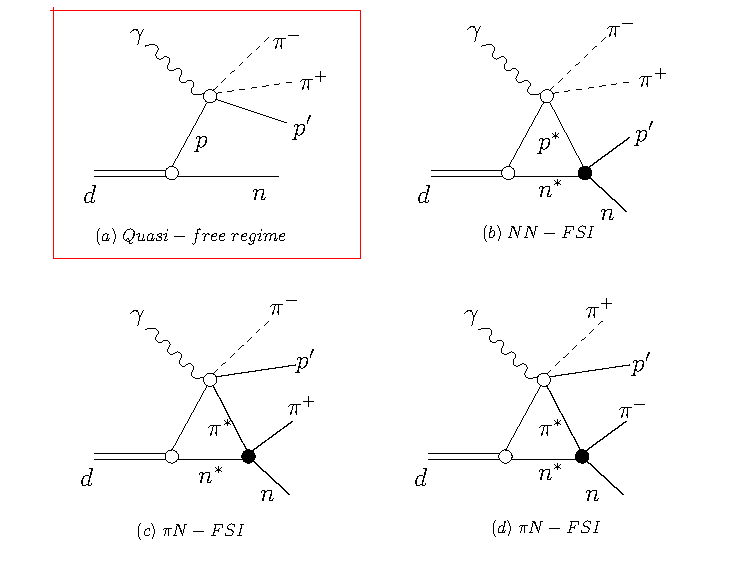
\includegraphics[width=\textwidth]{pictures/fsi_discuss/fsi_mech.pdf}}
\end{center}
\caption{\small Illustration of the leading contributors to the process of the double-pion production off the proton bound in deuteron. (a) Quasi-free regime, (b) NN-FSI, and (c-d) $\pi N$-FSI.}
\label{fig:fsi_mech}
\end{figure}


One mechanism of the proton-neutron scattering seems to be very interesting in the context of this study, i.e. the charge exchange mechanism, in which proton and neutron can exchange their characteristics, literally turning one into another. This may complicate the interpretation of the experimentally collected information. For example, some protons of the original exclusive reaction are not registered as they have undergone the exchange transformation to neutrons. Furthermore, some registered protons may turn out to be actually ``transformed'' neutrons from an exclusive reaction off neutrons bound in deuterium. 

The pion-nucleon scattering also involves a remarkable mechanism that deserves special attention, namely, the pion to neutron coupling with resonance formation. Section~\ref{Sect:resonance_fsi} of this chapter explores manifestations of this mechanism in the analyzed experimental data.


Among the main FSI components shown in Fig.~\ref{fig:fsi_mech}, proton-neutron interactions, which correspond to the process (b), are thought to dominate over the pion-neutron interactions, sketched in (c) and (d). Using the ``black disk" analogy, this ranking can be understood from the fact that a proton, being larger than a pion, has higher chances to spatially overlap with the neutron while traveling away from the vertex. In addition to that, due to the large difference in mass, protons and pions of a same momentum differ significantly in their velocity with the former being much slower. This makes the protons spend more time near the vertex (and hence near the neutron), which increases the interaction probability.


Due to the relatively low energy of the final hadrons, the majority of FSI in the investigated reaction are thought to happen elastically, which implies that (i) the quantum numbers of the participating hadrons do not change and (ii) no new particles are produced in such interactions. Note that the aforementioned mechanisms of the charge exchange in the proton-neutron scattering and the resonance formation in the process $\pi n \rightarrow \pi n$ are still attributed to elastic mechanisms. The minority of FSI in this reaction then evolves via inelastic scenarios~\cite{Shirokov_Yudin:1980}.  


The main goal of this study is to extract the double-pion cross sections in the quasi-free regime. Such an approach implies that quasi-free events that correspond to the process (a) in Fig.~\ref{fig:fsi_mech} are of interest, while events with FSI are treated as undesirable background and have to be eliminated. The analysis, therefore, was seeking special methods of separating these two types of events and correcting for the remaining admixture of events with FSI if the complete separation was not possible. These methods are described in detail in Sect.~\ref{Sect:excl_cut}.


Thus, being attributed to the background and hence subjected to elimination, events with FSI were deprived of attention throughout the analysis. These events, therefore, were lacking detailed investigation, which they definitely deserve as FSI effects represent an essential issue in studies of any exclusive reaction, especially off nuclei. To regain fairness and balance into the analysis, this particular chapter is fully focused on the events with FSI and is devoted to the discussion of their peculiar features and manifestations. 


\section{Probing FSI kinematically}

\everypar{\looseness=-1}
Recall that in general one can distinguish between two FSI types: (i) interactions between the final hadrons and (ii) interactions with spectator nucleons. These two FSI types, both driven by the strong interaction, seem to be similar to each other from the point of view of involved FSI mechanisms. Meanwhile, from the point of view of the reaction kinematics they differ. To discern this difference, let's consider each FSI type in more detail.


In general, all interactions that possibly could happen between the hadrons share the following three features,

\begin{itemize}
\item they preserve the total momentum of the participating hadrons, thus maintaining energy-momentum conservation between them,
\item after FSI the participating hadrons are left on their mass shell, and
\item the momentum of each participating hadron is altered and thus does not match its value before FSI.
\end{itemize}

These features deliver the following important conclusion: interactions between the final hadrons do not alter missing mass distributions\footnote[3]{If new particles are not produced in these interactions.}. As an interesting example, one can consider the situation when in a missing hadron topology FSI happens between a registered hadron and the unregistered one. In this case, the calculated four-vector of a missing particle matches its actual four-momentum after FSI (in the absence of other factors, such as detector resolution, radiative effects, etc.) because the interaction keeps the energy-momentum conservation between the reaction particles. Then, as the unregistered particle ends up being on-shell after FSI, the calculated missing mass turns out to match the particle rest mass.

Although having no impact on the missing mass distributions, FSI between final hadrons nonetheless affect the experimentally extracted cross sections. This happens due to the following reason. Let's suppose that in the reaction of the double-pion production, two final hadrons interact with each other, while the third one avoids any interactions. In this case, the two interacting hadrons change their four-momenta (keeping their cumulative momentum unchanged though), while the third one manages to reach the detector unaltered. Then, for such an event, the calculated final hadron variables will differ from their true values before FSI. Specifically, the invariant mass of the pair of interacting hadrons will be preserved (due to the conservation of their cumulative four-momentum), whereas the invariant masses of an interacting hadron and the unaltered one will change. Moreover, the spatial angles of the unaltered hadron will be preserved, whereas the angles of both interacting hadrons will change. Such an event then will contribute to the ``wrong'' point of the reaction phase-space that is different from the point it is supposed to contribute without FSI. As a result, the measured cross sections acquire disturbances.


\everypar{\looseness=-1}
This issue with the cross section disturbances can hardly be avoided on the level of the experimental data analysis due to the insensitivity of the missing mass distributions to interactions of the final hadrons with each other. Therefore, measured cross sections (no matter whether off a free or bound nucleon) are inevitably convoluted with effects of this FSI type. This issue is supposed to be treated on the level of theoretical/phenomenological cross section interpretation.



Meanwhile, FSI with spectator nucleons have one distinctive feature, which differentiate them from FSI between the final hadrons. Specifically, as the spectator nucleon is extrinsic to the original exclusive reaction, any FSI with it causes in/out momentum flows, thus breaking the energy-momentum conservation imposed on the reaction particles. This means that after FSI the total energy/momentum of the reaction final hadrons is different from what they had before FSI as some part of it was either given to or taken from the neutron. As a consequence, for events with FSI, the missing mass technique gives faulty results for both the fully exclusive event sample or the one with a missing hadron, which means that FSI with the spectator introduce disturbances into the missing mass distributions.


Note that interactions between one of the final hadrons and the spectator neutron should anyway comply with the three above features, which implies not only the energy-momentum conservation in this particular interaction, but also the on-shellness of both interacting particles after the interaction happens.


The revealed specificity of FSI with spectator neutrons (i.e. the ability to disturb missing mass distributions), allows for a kinematic probing of this FSI type, which is unfortunately not possible for the case of final hadrons interacting with each other. Seeking to exploit this unique opportunity offered by ``e1e" deuteron target experiment, the rest of this chapter is devoted to the kinematic examination of FSI with spectator nucleons in the reaction of the double-pion electroproduction off protons bound in deuterium nuclei. This implies that hereinafter whenever FSI is mentioned, the processes (b-d) of Fig.~\ref{fig:fsi_mech} are assumed unless specified otherwise.


It is convenient to start kinematic probing of FSI by recalling a few general facts. 


First, it is worthwhile to recall that the amount of events produced in an exclusive reaction depends on a certain number of independent variables, which in the case of double-pion electroproduction is seven as described in Sect.~\ref{Sect:kin_var}. The yields of quasi-free events and events with FSI represent complementary portions of the total number of reaction events, and hence both of them depend on these variables as well. Therefore, it is reasonable to consider the relative spread of events with FSI, which implies that the amount of events affected by FSI in any part of the reaction phase space is analyzed with respect to the corresponding amount of quasi-free events.


\everypar{\looseness=-1}
Meanwhile, the portion of events with FSI is not expected to be the same along the reaction phase space. Instead, their relative spread is anticipated to rise in the region of small hadron momenta as slower traveling hadrons have higher interaction probability. Meanwhile, in the acceptance of the CLAS detector the region of large polar angles corresponds mostly to low-momentum hadrons\footnote[4]{The mentioned correlation between the momentum and the polar angles of the final hadrons can be observed in the $\theta$ versus momentum distributions provided in Sect.~\ref{Sect:fiduc}. }. Therefore, a relative excess of events with FSI is also expected with increasing hadron polar angles. In addition to that, as various reaction topologies cover different ranges of hadron momenta and angles, the relative spread of events with FSI acquires topology dependence. 

\everypar{\looseness=-1}
It is also important to emphasize that in general final state interactions are very complicated and involve numerous mechanisms. Their complete theoretical description requires application of the theory of the strong interactions and so far is not fully accomplished. However, all mechanisms that possibly could happen during FSI have one simple feature in common, i.e. they alter the momentum of the participating hadrons.


With regards to alterations of hadron momenta in collisions with the spectator neutrons, the following kinematic aspects should be taken into consideration. The neutrons move with the Fermi momentum, which for the vast majority of events is less than $\sim$250~MeV, but rarely can be higher. Meanwhile, in the analyzed experiment, the momentum of all final hadron types can be as high as $\sim$1.5~GeV. Therefore, in collisions with neutrons, rapid final hadrons are expected to mostly lose their momentum, whereas for slow hadrons a momentum gain is quite likely to occur. Here one should also take into account that due to the presence of registration thresholds, pions slower than $\sim$100~MeV and protons slower than $\sim$300~MeV are not registered.


Now, having highlighted important general facts, it is worthwhile to recapitulate those features of FSI with spectator nucleons, which form the basis of the kinematic examination of FSI effects presented further in this chapter. Specifically, FSI with spectator nucleons (i) alter the momentum of the participating particles and (ii)~do not preserve energy-momentum conservation between the final hadrons of the initial exclusive reaction. As a result, distributions of kinematic quantities calculated~from the registered final hadron four-momenta acquire disturbances caused by agglomerations of events with FSI. These disturbances can be better visually~distinguished, if the corresponding distributions of pure quasi-free events are used as reference. 


The outlined effect was already exploited in this analysis on the quasi-free event selection level as described in detail in Sect.~\ref{Sect:excl_cut}. The disturbances caused by events with FSI were observed in the distributions of missing quantities $P_{X}$, $M^{2}_{X[0]}$, and $M^{2}_{X[\pi^{-}]}$, which were used to establish the exclusivity cuts. However, the examination conducted in Sect.~\ref{Sect:excl_cut} was mostly concentrated on quasi-free events as they were the main point of interest for the analysis, while events with FSI lacked consideration. In this chapter, the distributions of missing quantities are examined once again with attention focused on FSI induced disturbances.


The two reaction topologies are again considered separately as FSI effects turn out to be topology dependent. The fully exclusive topology is addressed first as it benefits from capturing FSI for all three final hadrons including the $\pi^{-}$. 


\section{FSI in the fully exclusive topology}
\subsection{Relative spread of FSI events along the phase space }

For the fully exclusive topology, the distributions of the following quantities are examined\footnote[5]{The quantity $M^{2}_{X[0]}$ is not examined here as it was shown in Ref.~\cite{note_mm_distr} to be quite insensitive to FSI with spectator nucleons.}: the missing momentum $P_{X}$ for the reaction $ep(n)\rightarrow e'p'(n')\pi^{+}\pi^{-}X$ and the missing mass squared $M^{2}_{X[\pi^{-}]}$ for the reaction $ep(n)\rightarrow e'p'(n')\pi^{+}X$. These quantities are defined by\vspace{-1.25em}
\begin{equation}
\begin{aligned}
&P_{X}&=&~|\overrightarrow{P}_{e} - \overrightarrow{P}_{e'}- \overrightarrow{P}_{p'} - \overrightarrow{P}_{\pi^{+}} - \overrightarrow{P}_{\pi^{-}}|,\\[-3pt]
&M_{X[\pi^{-}]}^{2}&=&~[P_{\pi^{-}~miss}^{\mu}]^{2}=[P_{e}^{\mu} + P_{p}^{\mu}- P_{e'}^{\mu}- P_{p'}^{\mu}-  P_{\pi^{+}}^{\mu}]^{2},\\[-10pt]
\end{aligned}\label{eq:excl_top_quant2}
\end{equation}%\vspace{-1em}
where $P_{i}^{\mu}$ are the four-momenta and $\overrightarrow{P_{i}}$ the three-momenta of the particle $i$. Both quantities are calculated under the target-at-rest-assumption, i.e. considering $P^{\mu}_{p} = (0,~0,~0,~m_{p})$, where $m_{p}$ is the proton mass.

As reference distributions of pure quasi-free events, the distributions of the same quantities plotted for the Monte Carlo simulation are used. The Monte Carlo simulation was performed on the basis of the TWOPEG-D event generator~\cite{twopeg-d}, which nicely reproduces the Fermi smearing of the missing quantities, but does not include FSI effects. The comparison of the FSI disturbed experimental distributions with these reference histograms reveals the features of events with FSI. 


In the first step, the relative spread of events with FSI along the magnitude of the final hadron momenta is examined. Figures~\ref{fig:fsi_mom_dep_pim},~\ref{fig:fsi_mom_dep_pip}, and~\ref{fig:fsi_mom_dep_pr} show the distributions of the quantities $P_{X}$ (first row) and $M^{2}_{X[\pi^{-}]}$ (second row) plotted in different ranges of $\pi^{-}$, $\pi^{+}$, and proton momentum magnitudes, respectively. The relative spread of events with FSI can be visually judged by the mismatch between the experimental (black) and simulated (blue) histograms. The considered ranges of the hadron momenta are specified for each plot. Note that these ranges are not equidistant and were chosen in such a way that the relative amount of events with FSI does not change significantly within each range. The distributions are plotted for events from the fully exclusive topology and normalized in a way that the maxima of the main peaks are equal~to~one. 

As follows from Fig.~\ref{fig:fsi_mom_dep_pim}, events with low $\pi^{-}$ momenta ($\lesssim$~0.5~GeV) contain a considerable fraction of events with FSI, while events with higher $\pi^{-}$ momenta ($\gtrsim$~0.5~GeV) are mostly quasi-free. However, the relative spread of events with FSI along the $\pi^{+}$ momentum demonstrates a different tendency as shown in Fig.~\ref{fig:fsi_mom_dep_pip}, i.e. the fraction of events with FSI does not vary significantly along the $\pi^{+}$ momentum, staying sizable for all momentum values.

%\newpage
\afterpage{\clearpage}
\begin{figure}[!ht]
\begin{center}
\framebox{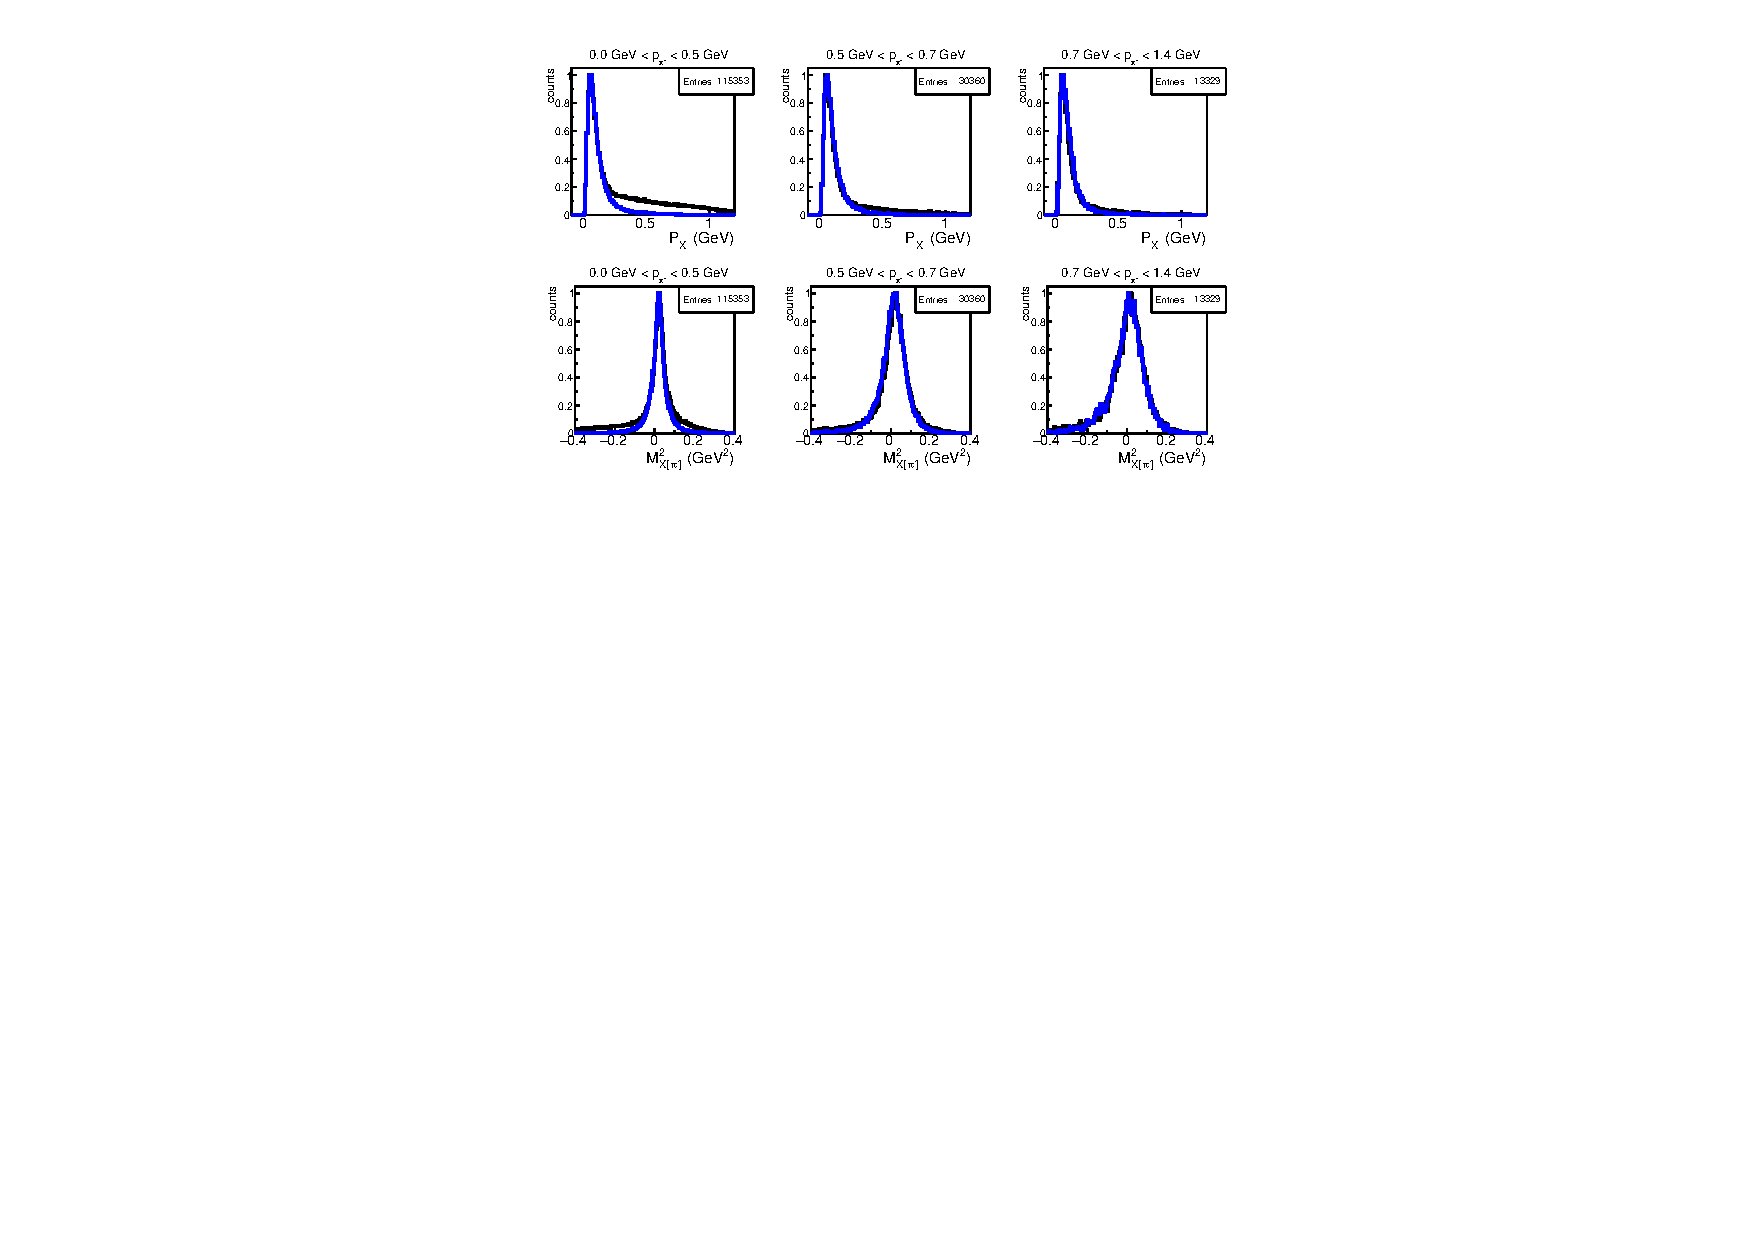
\includegraphics[trim=0 0 8cm 0, clip=true, width=0.6\textwidth]{pictures/fsi_discuss/mom_dep_pim.pdf}}
\end{center}
\caption{\small Relative spread of events with FSI among different ranges of the $\pi^{-}$ momentum magnitude is demonstrated by the mismatch between the experimental (black) and the simulated (blue) distributions of the quantities $P_{X}$ (first row) and $M^{2}_{X[\pi^{-}]}$ (second row) defined by Eqs.~\eqref{eq:excl_top_quant2}. The corresponding ranges of the $\pi^{-}$ momentum are specified above the plots. Note that these ranges are not equidistant and were chosen in a way that the relative amount of events with FSI does not change significantly within each range. The distributions are plotted for events from the fully exclusive topology and normalized in a way that the maxima of the main peaks are equal to one. The presented statistics corresponds to the experimental data.}
\label{fig:fsi_mom_dep_pim}
\end{figure}


\begin{figure}[!ht]
\begin{center}
\framebox{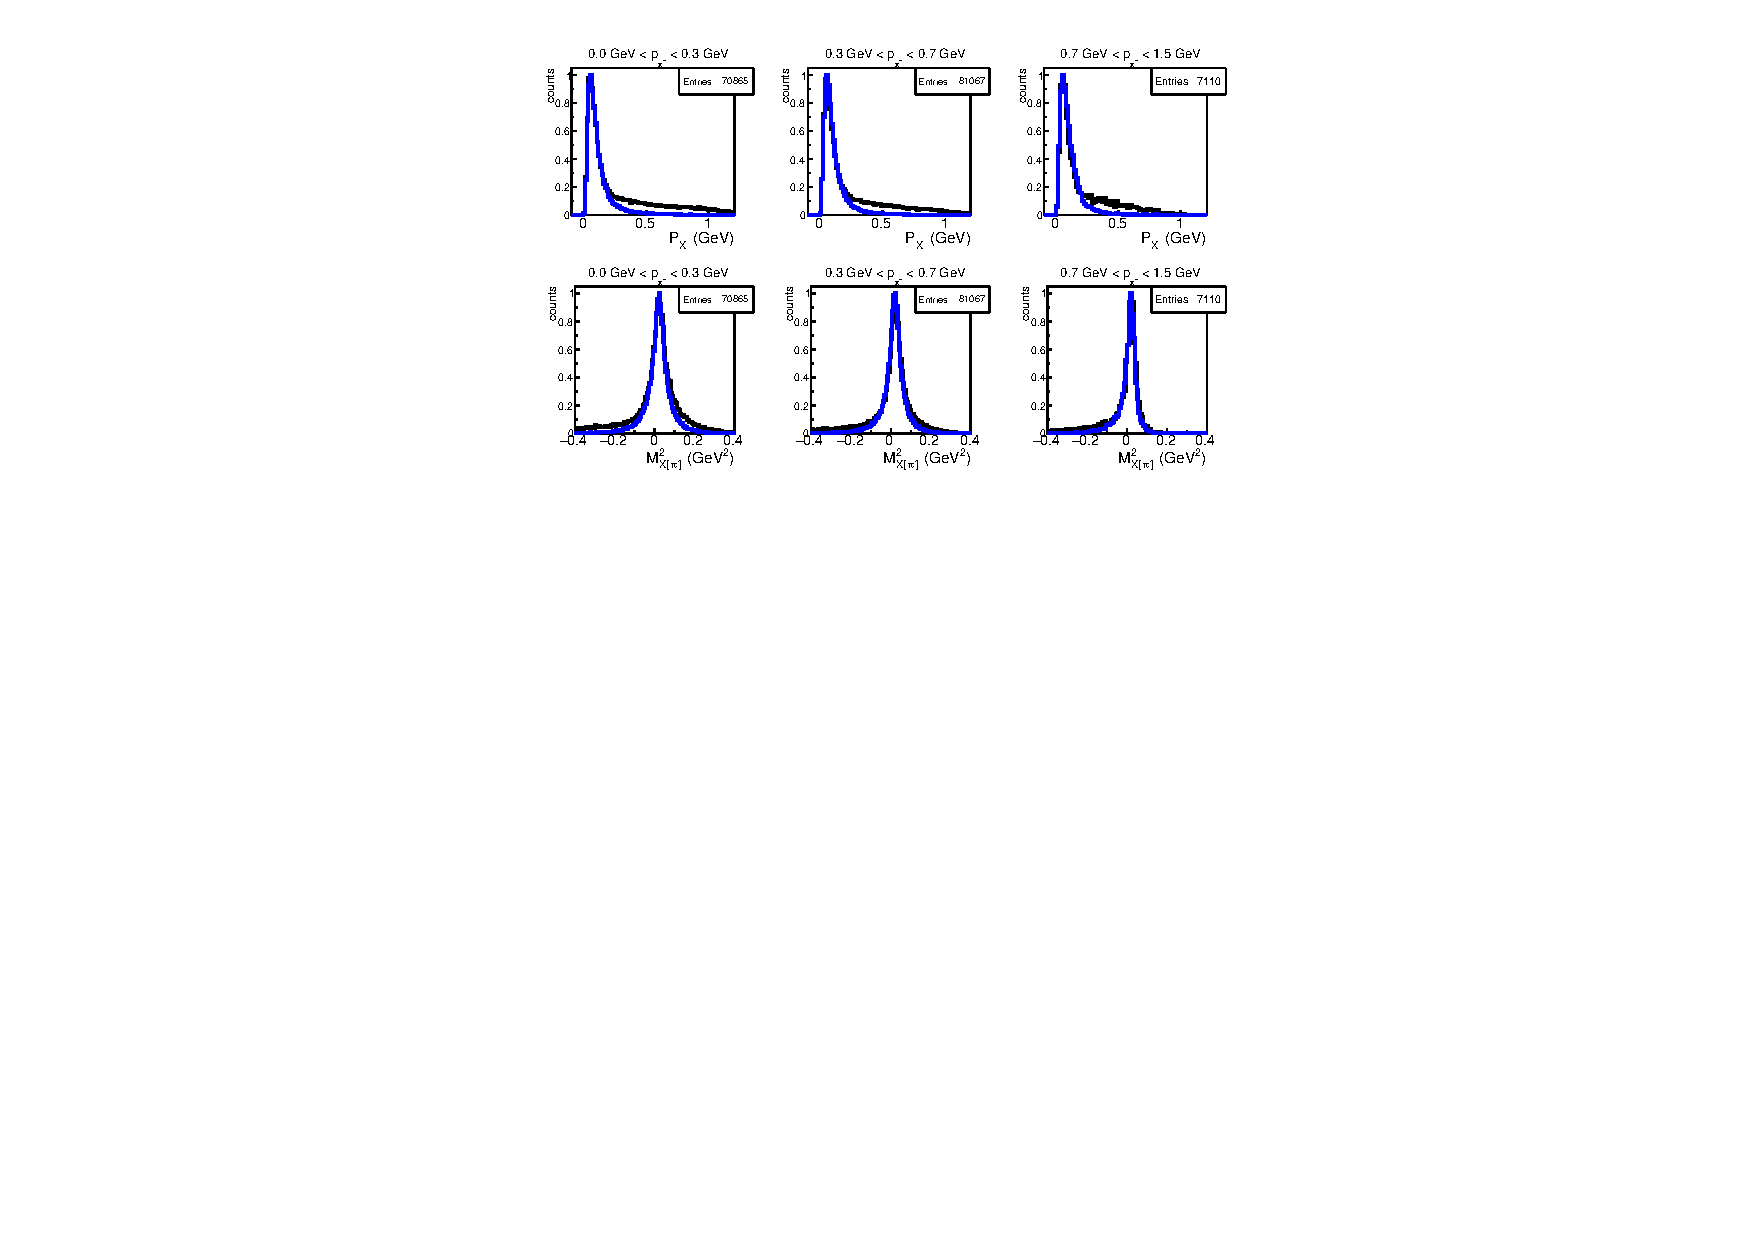
\includegraphics[trim=0 0 8cm 0, clip=true, width=0.6\textwidth]{pictures/fsi_discuss/mom_dep_pip.pdf}}
\end{center}
\caption{\small Relative spread of events with FSI among different ranges of the $\pi^{+}$ momentum magnitude is demonstrated by the mismatch between the experimental (black) and the simulated (blue) distributions of the quantities $P_{X}$ (first row) and $M^{2}_{X[\pi^{-}]}$ (second row) defined by Eqs.~\eqref{eq:excl_top_quant2}. The corresponding ranges of the $\pi^{+}$ momentum are specified above the plots. Note that these ranges are not equidistant and were chosen in a way that the relative amount of events with FSI does not change significantly within each range. The distributions are plotted for events from the fully exclusive topology and normalized in a way that the maxima of the main peaks are equal to one. The presented statistics corresponds to the experimental data.}
\label{fig:fsi_mom_dep_pip}
\end{figure}
\begin{figure}[!ht]
\begin{center}
\framebox{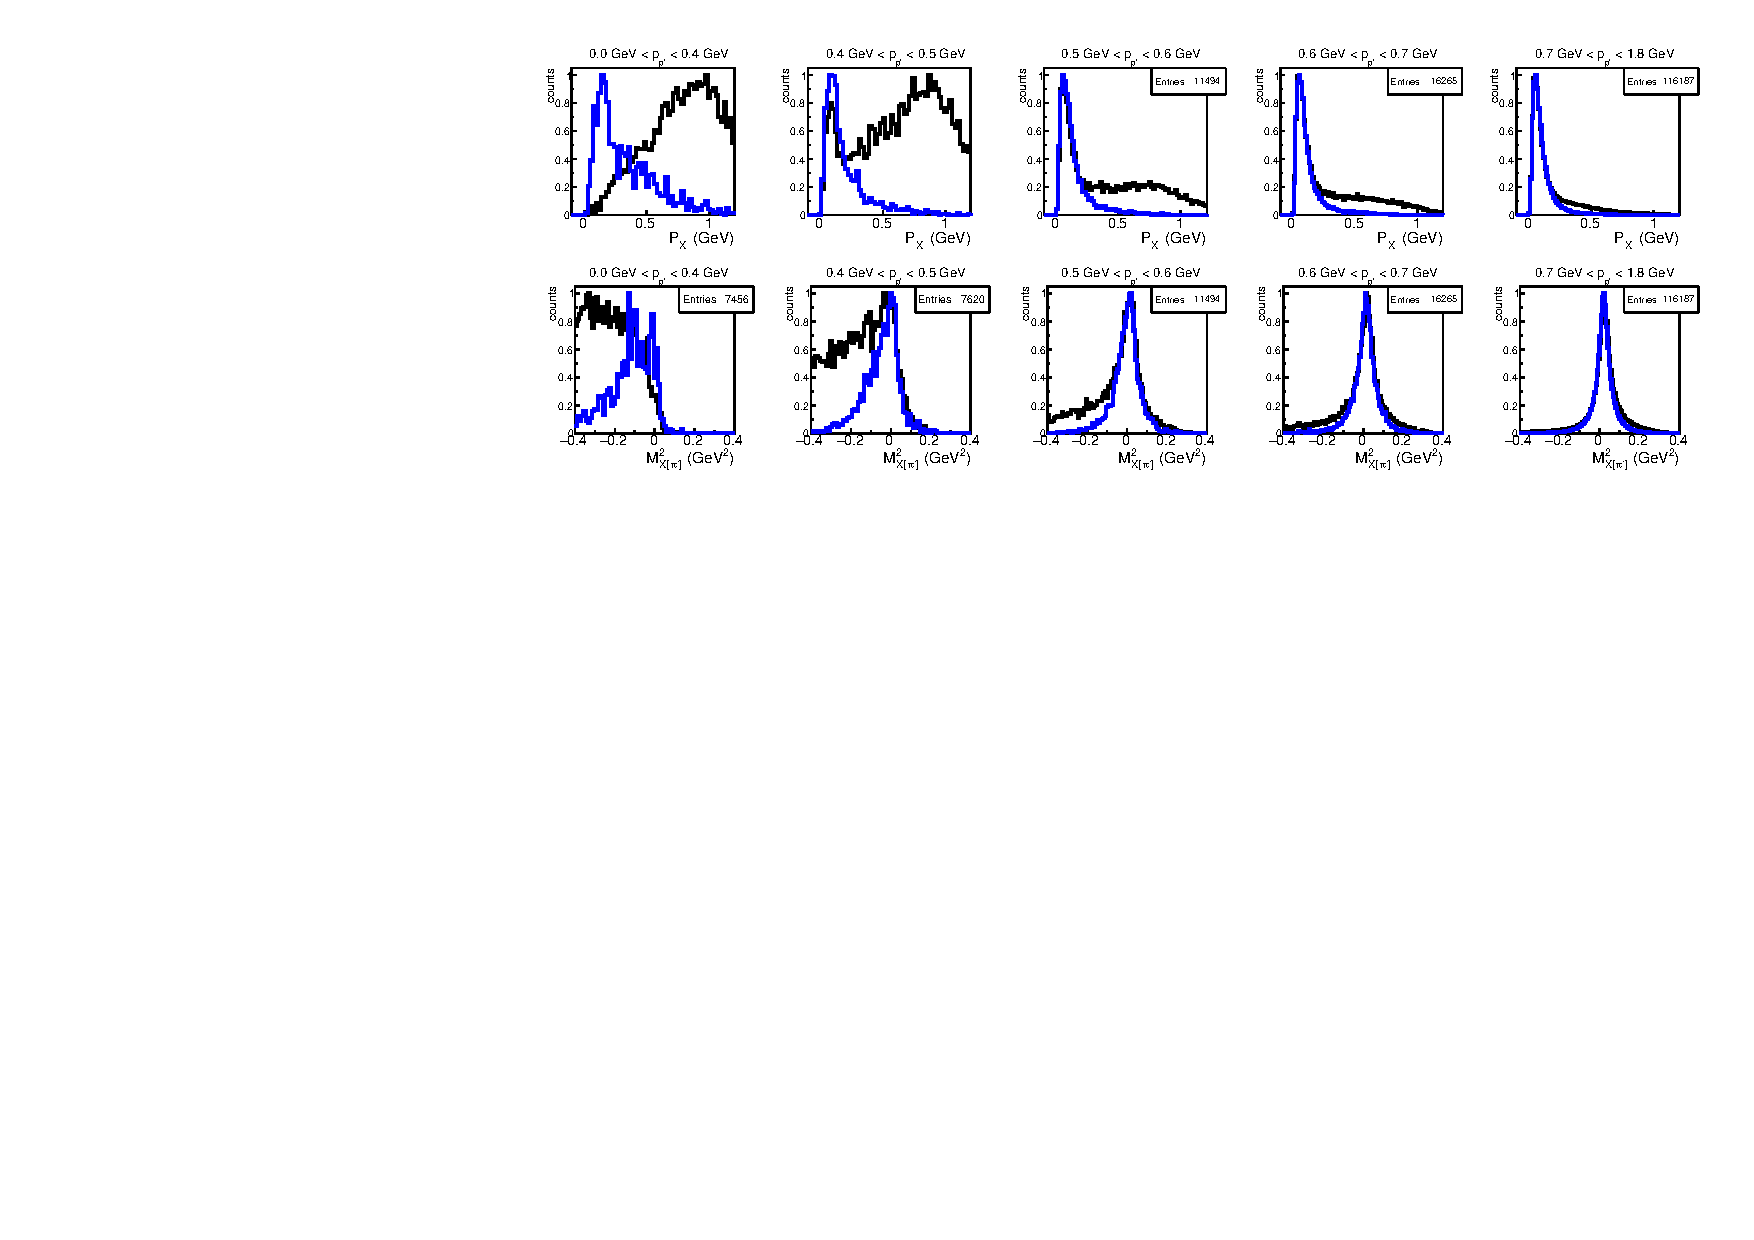
\includegraphics[width=\textwidth]{pictures/fsi_discuss/mom_dep_pr.pdf}}
\end{center}
\caption{\small Relative spread of events with FSI among different ranges of the proton momentum magnitude is demonstrated by the mismatch between the experimental (black) and the simulated (blue) distributions of the quantities $P_{X}$ (first row) and $M^{2}_{X[\pi^{-}]}$ (second row) defined by Eqs.~\eqref{eq:excl_top_quant2}. The corresponding ranges of the proton momentum are specified above the plots. Note that these ranges are not equidistant and were chosen in a way that the relative amount of events with FSI does not change significantly within each range. The distributions are plotted for events from the fully exclusive topology and normalized in a way that the maxima of the main peaks are equal to one. The presented statistics corresponds to the experimental data.}
\label{fig:fsi_mom_dep_pr}
\end{figure}

%\newpage
Meanwhile, the relative spread of events with FSI varies dramatically along the proton momentum as illustrated by Fig.~\ref{fig:fsi_mom_dep_pr}. In the region of low proton momenta $\lesssim$~0.4~GeV no quasi-free events are present\footnote[6]{Note that in this region an admixture of spectator protons from the reaction off neutrons may~be present. Also, in CLAS, reconstruction of protons with $p_{p'}\lesssim~0.4~$GeV is in general not quite~reliable.}. As the proton momentum grows up to $\sim$0.5~GeV quasi-free events begin to appear in the sample, which is however still dominated by events with FSI. Then, in the region $\gtrsim$~0.5~GeV quasi-free events begin to prevail, but the fraction of events with FSI is still essential up to the values of $\gtrsim$~0.6~GeV. As the proton momentum grows further, the admixture of events with FSI is mitigated and for the values $\gtrsim$~0.7~GeV mostly quasi-free events are left.


\begin{figure}[!ht]
\begin{center}
\framebox{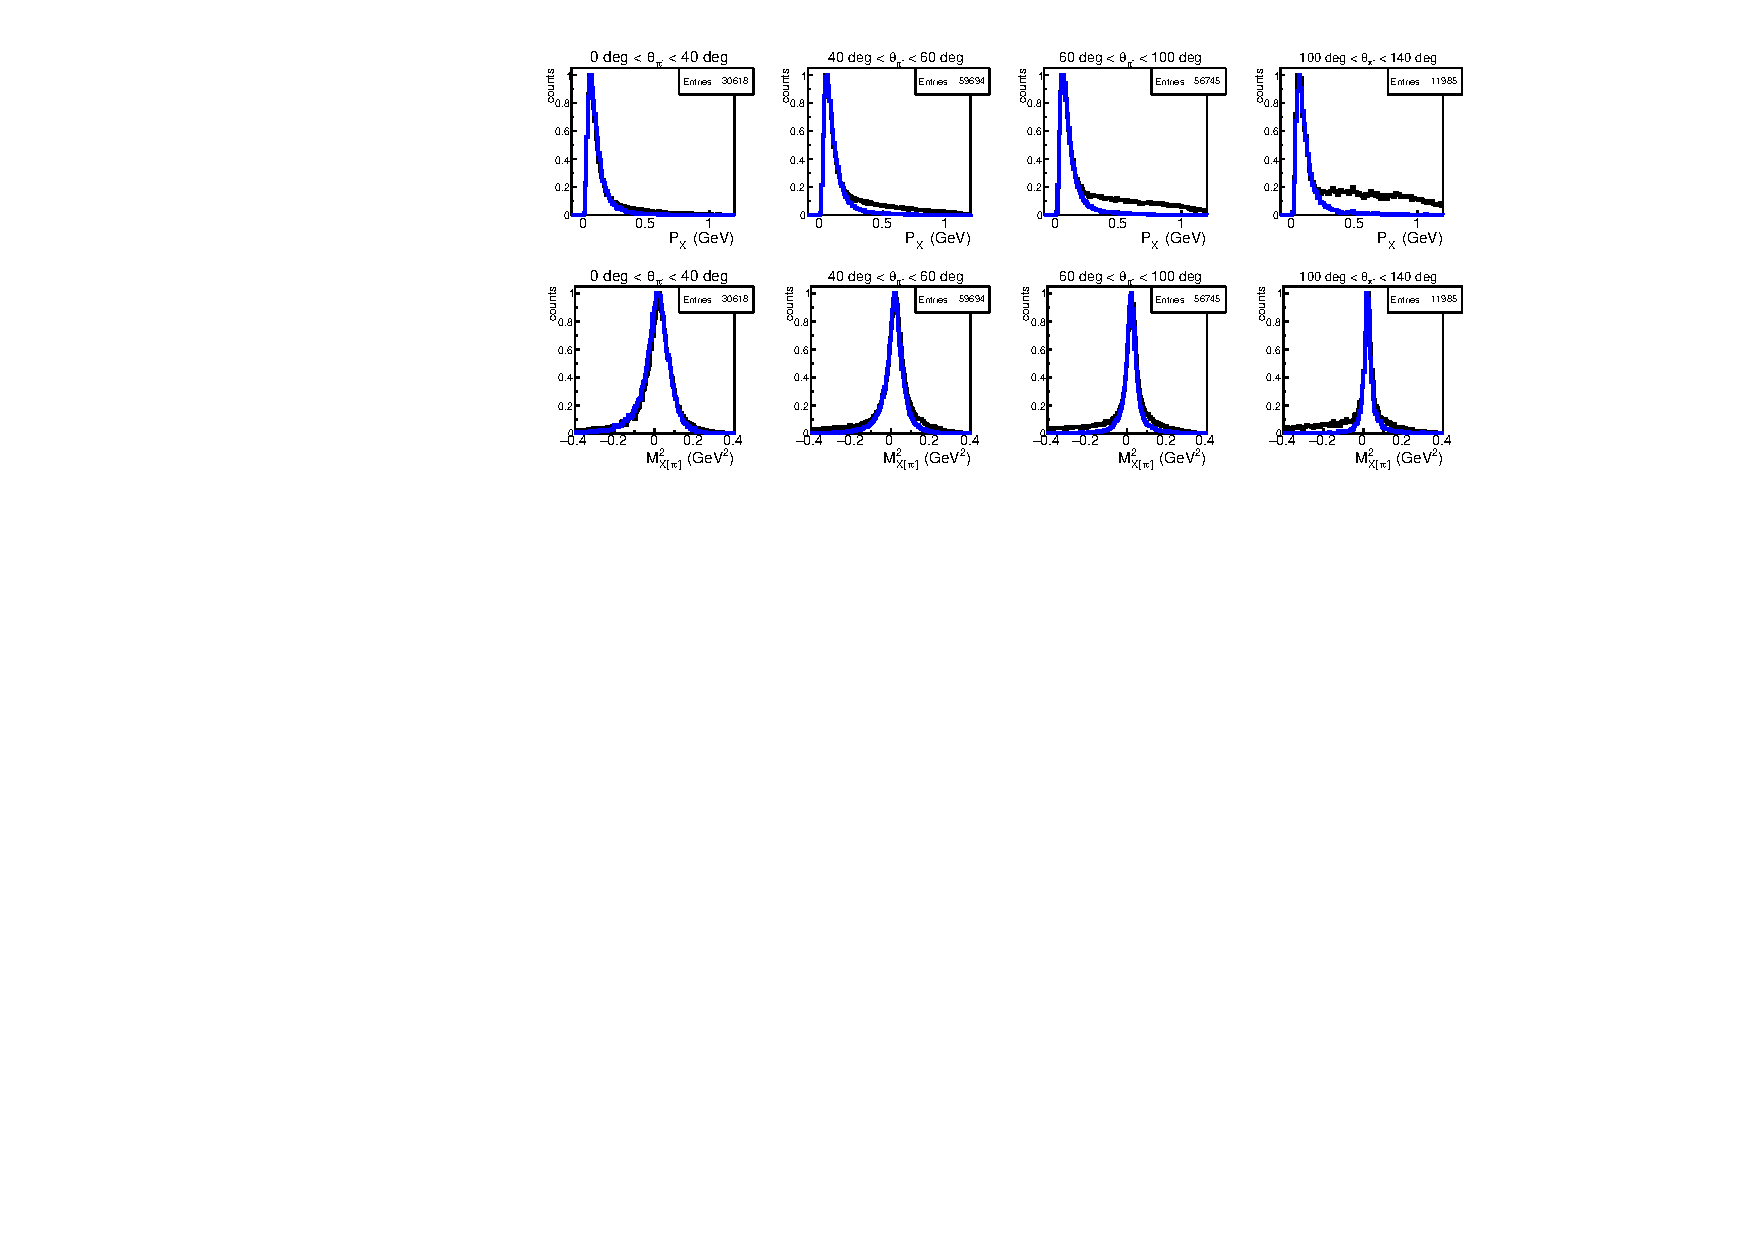
\includegraphics[trim=0 0 4cm 0, clip=true, width=0.8\textwidth]{pictures/fsi_discuss/th_dep_pim.pdf}}
\end{center}
\caption{\small Relative spread of events with FSI among different ranges of the $\pi^{-}$ polar angle is demonstrated by the mismatch between the experimental (black) and the simulated (blue) distributions of the quantities $P_{X}$ (first row) and $M^{2}_{X[\pi^{-}]}$ (second row) defined by Eqs.~\eqref{eq:excl_top_quant2}. The corresponding ranges of the $\pi^{-}$ polar angle are specified above the plots. Note that these ranges are not equidistant and were chosen in a way that the relative amount of events with FSI does not change significantly within each range. The distributions are plotted for events from the fully exclusive topology and normalized in a way that the maxima of the main peaks are equal to one. The presented statistics corresponds to the experimental data.}
\label{fig:fsi_th_dep_pim}
\end{figure}

In the next step, the relative spread of events with FSI along the polar angle of the final hadrons is examined in the same way. Figures~\ref{fig:fsi_th_dep_pim},~\ref{fig:fsi_th_dep_pip}, and~\ref{fig:fsi_th_dep_pr} show the distributions of the quantities $P_{X}$ (first row) and $M^{2}_{X[\pi^{-}]}$ (second row) plotted in different ranges of $\pi^{-}$, $\pi^{+}$, and proton polar angle, respectively. The relative spread of events with FSI is again demonstrated by the mismatch between the experimental (black) and simulated (blue) histograms and the considered ranges of hadron polar angles are specified for each plot. These ranges are again not equidistant and as they were chosen in such a way that the relative amount of events with FSI does not change significantly within each range. %The distributions are plotted for events from the fully exclusive topology and normalized in a way that the maxima of the main peaks are equal to one. 

\afterpage{\clearpage}

%\newpage
\begin{figure}[!ht]
\begin{center}
\framebox{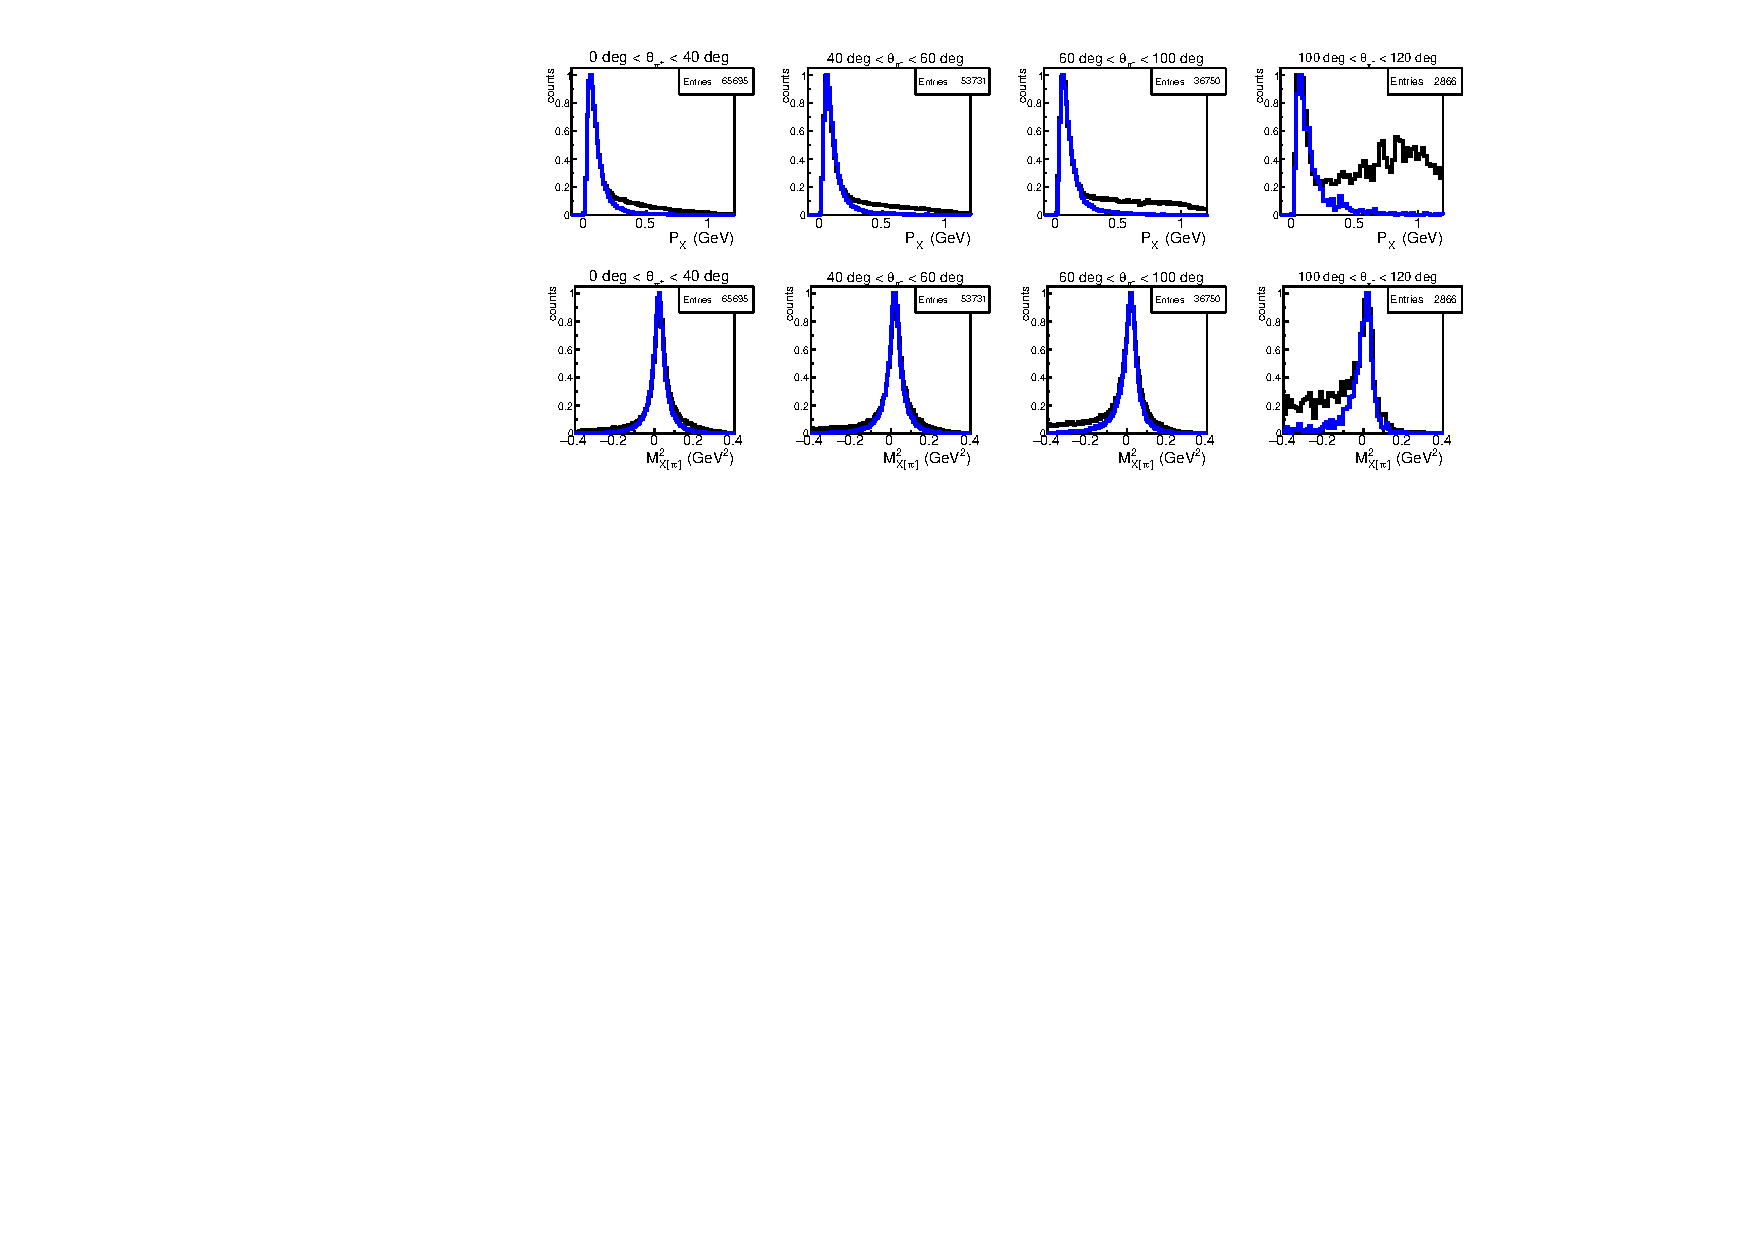
\includegraphics[trim=0 0 4cm 0, clip=true, width=0.8\textwidth]{pictures/fsi_discuss/th_dep_pip.pdf}}
\end{center}
\caption{\small Relative spread of events with FSI among different ranges of the $\pi^{+}$ polar angle is demonstrated by the mismatch between the experimental (black) and the simulated (blue) distributions of the quantities $P_{X}$ (first row) and $M^{2}_{X[\pi^{-}]}$ (second row) defined by Eqs.~\eqref{eq:excl_top_quant2}. The corresponding ranges of the $\pi^{+}$ polar angle are specified above the plots. Note that these ranges are not equidistant and were chosen in a way that the relative amount of events with FSI does not change significantly within each range. The distributions are plotted for events from the fully exclusive topology and normalized in a way that the maxima of the main peaks are equal to one. The presented statistics corresponds to the experimental data.}
\label{fig:fsi_th_dep_pip}
\end{figure}
\begin{figure}[!ht]
\begin{center}
\framebox{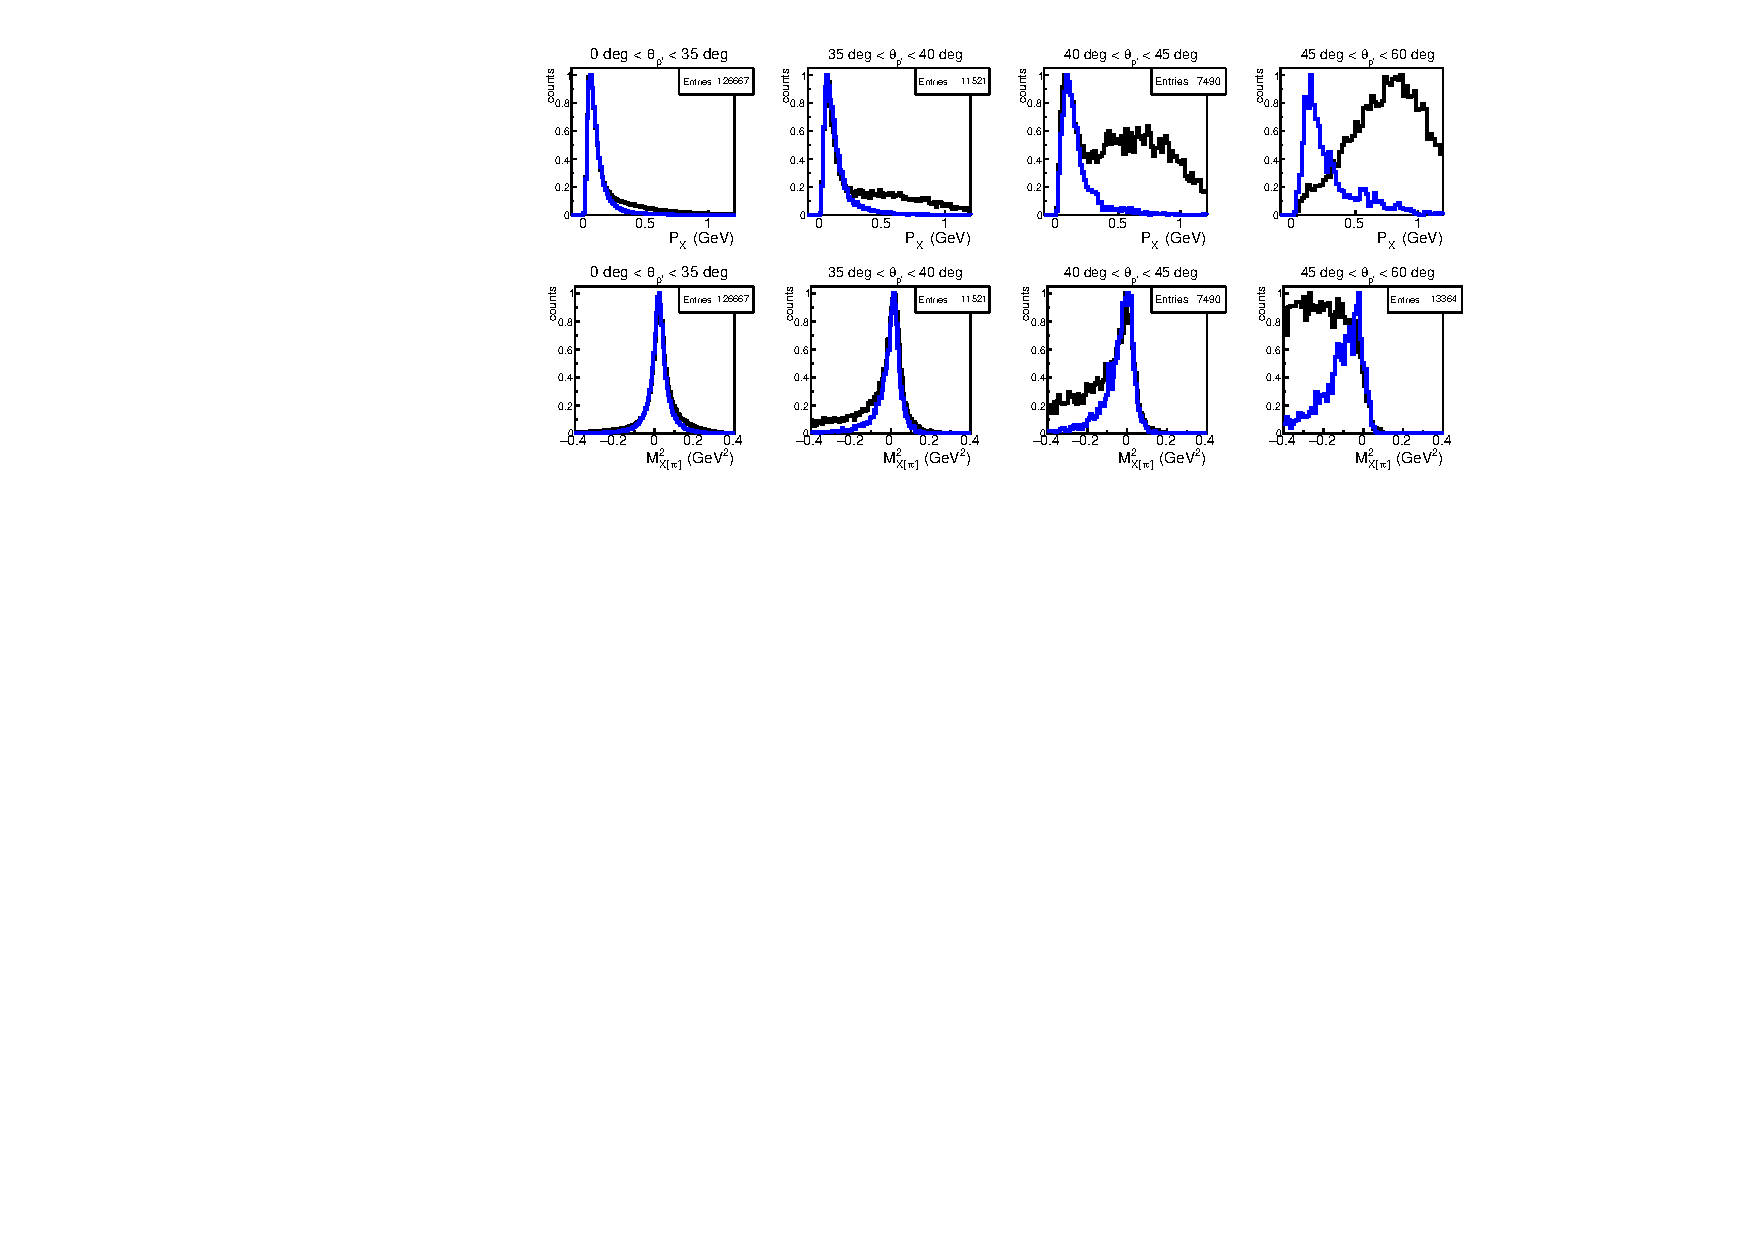
\includegraphics[trim=0 0 4cm 0, clip=true, width=0.8\textwidth]{pictures/fsi_discuss/th_dep_pr.pdf}}
\end{center}
\caption{\small Relative spread of events with FSI among different ranges of the proton polar angle is demonstrated by the mismatch between the experimental (black) and the simulated (blue) distributions of the quantities $P_{X}$ (first row) and $M^{2}_{X[\pi^{-}]}$ (second row) defined by Eqs.~\eqref{eq:excl_top_quant2}. The corresponding ranges of the proton polar angle are specified above the plots. Note that these ranges are not equidistant and were chosen in a way that the relative amount of events with FSI does not change significantly within each range. The distributions are plotted for events from the fully exclusive topology and normalized in a way that the maxima of the main peaks are equal to one. The presented statistics corresponds to the experimental data.}
\label{fig:fsi_th_dep_pr}
\end{figure}

%----------------------------------------------


As follows from Fig.~\ref{fig:fsi_th_dep_pim}, events with low values of the $\pi^{-}$ polar angle $\lesssim$~40$^{\circ}$ are mostly quasi-free, while in the region $\gtrsim$~40$^{\circ}$ a discernible fraction of events with FSI appears. This fraction gradually grows with increasing polar angle and in the region of $120^{\circ}<\theta_{\pi^{-}}<140^{\circ}$ becomes considerable. 

The relative spread of events with FSI along the $\pi^{+}$ polar angle again demonstrates a slightly different tendency, as seen in Fig.~\ref{fig:fsi_th_dep_pip}. The fraction of events with FSI turns out to be discernible for all values of the $\pi^{+}$ polar angle, showing a mild growth as the angle increases up to 100$^{\circ}$. Then, in the region of $100^{\circ}<\theta_{\pi^{+}}<120^{\circ}$ the number of events with FSI rises suddenly up to a rather essential portion.

The correlation between the fraction of events with FSI and the proton polar angle is again more dramatic. As seen in Fig.~\ref{fig:fsi_th_dep_pr}, in the region $\theta_{p}<35^{\circ}$, which contains the majority of registered protons, the portion of events with FSI is discernible but small. However, for higher polar angles a rather steep rise of this portion takes place, i.e. in the narrow slice of $35^{\circ}<\theta_{p}<40^{\circ}$ it becomes considerable and in the next $5^{\circ}$-range -- very large. Finally, for $\theta_{p}>45^{\circ}$ quasi-free events turn out to vanish, while events with FSI prevail.


The examination performed above confirms the expected increase in the relative amount of events with FSI in the regions of low momentum and large polar angles, which is observed for all final hadrons, to one extent or another. The anticipated dominance of proton-neutron interactions over the pion-neutron interactions is also in agreement with the observations. In addition to these general statements, the following more specific conclusions can be made.%\vspace{-0.3em}
\begin{itemize}
\item The fraction of events with FSI is strongly correlated with the proton kinematics, giving steep rises in the low-momentum region as well as for the region of large polar angles.%\vspace{-0.125em}
\item The correlation with the $\pi^{-}$ kinematics is mild with no steep alterations seen.%\vspace{-0.125em}
\item The correlation with the $\pi^{+}$ kinematics is quite weak, with the only one exception of an essential rise for $\theta_{\pi^{+}}>100^{\circ}$. %\vspace{-0.125em}
\item In the regions of the $\pi^{-}$ momentum $\gtrsim$~0.5~GeV and the $\pi^{-}$ polar angle $\lesssim 40^{\circ}$ the event sample is completely dominated by quasi-free events.%\vspace{-0.125em}
\item In the regions of the proton momentum $\lesssim$~0.4~GeV and the proton polar angle $\gtrsim 45^{\circ}$ the event sample is completely dominated by events with FSI.%\vspace{-0.35em}
\end{itemize}

\everypar{\looseness=-1}
Note that the above observations are to a high degree determined by experimental conditions, as for instance, by the hardware threshold on the minimal detectable hadron momenta, which affects manifestations of proton and pion FSI in a different way. The point is that protons and pions that carry equal momenta differ significantly in their velocity: the former turn out to be much slower than the latter due to the difference in their mass. As a result, pions with potentially high probability of FSI have a tendency to be located in the region of extremely low momenta, which lies below the registration threshold. Meanwhile, protons with high probability of FSI turn out to be located in the region of moderately low momenta, comparable with the threshold value. Thus, the majority of pions that experienced FSI failed to be registered, while for protons the situation is different as the large number of them cross the threshold and hence managed to be registered. 

\everypar{\looseness=-1}
The following several aspects are also noteworthy in the examination described above. First, the examination was performed for hadron momenta and polar angles defined in the laboratory system because this system is the only one that offers a sensible, unambiguous, and the most accurate determination of these quantities for events with FSI (which here are the main focus of interest). The arguments for this statement are given below.

The point is that the typically performed transformation to the CMS remains sensible only for quasi-free events, while for events with FSI it is no longer relevant. This happens because once participating in FSI, events do not further keep the kinematics of the initial reaction and hence formally do not belong to ``reaction events" anymore as in fact they were not produced off the target proton that defines the reaction CMS. Therefore, the usual CMS turns out to be an ill-defined system for events with FSI, and the transformation to this system would introduce further ambiguity into the examination. 

In addition to that, the proper transformation to the reaction CMS requires the knowledge of the Fermi momentum of the initial proton for each event. The fully exclusive topology in general allows the reconstruction of this momentum as missing, which actually outputs the quantity $P_{X}$. However, being reconstructed in such a way this momentum not only suffers from poor resolution, but is also in fact incorrect for events with FSI as their initial kinematics is altered. Another option, i.e. performing the transformation under the target-at-rest assumption, convolutes the transformed quantities with effects of the target motion and hence lacks enough accuracy as well\footnote[7]{For the purpose of calculating quasi-free cross sections in the main analysis this option was considered adequate as it was accompanied by the corresponding correction. See Sects.~\ref{Sect:lab_cms} and~\ref{Sect:fermi_corr}.}. Therefore, being transformed to CMS, hadron momenta and angles would acquire an unnecessary systematic uncertainty, which would tangle the examination.

Taking into account all above arguments, the laboratory system was considered to give the best possible opportunity for the examination of features and manifestations of FSI effects.

\everypar{\looseness=-1}
The performed examination was conducted on a qualitative level without giving any definitive quantitative conclusions on the observed percentage of events with FSI in the analyzed event sample. This examination style is determined by the fact that the interrelation between the quasi-free events and events with FSI is strongly dependent on experimental conditions, detector acceptance/efficiency, the chosen reaction topology, the event selection employed in the analysis, etc. Therefore, any quantitative conclusion on the revealed ratio of quasi-free and FSI-affected events would have been very condition-specific and thus misleading. Meanwhile, general tendencies observed in the spreading of FSI events along the reaction phase-space are thought to be more universal and stable, and therefore gain the main focus of this kinematic examination. 

\everypar{\looseness=-1}
Meanwhile, sensible quantitative conclusions on this matter should be established on the cross section level other than on a level of event yields. An excellent opportunity to achieve this goal opens up with the completion of this analysis as now the newly extracted quasi-free cross sections can be compared with the analogous double-pion cross sections off free protons obtained in Ref.~\cite{Fed_an_note:2017,Fed_paper_2018}. In this way, a condition-independent impartial  estimation of the relative contribution of events with FSI to the total amount of reaction events can be made. %This promising comparison is scheduled to follow this analysis.



\subsection{Revealing details on hadron momentum alterations}

Another noteworthy aspect of the performed examination is that one should be careful when considering the amount of events that fall within a certain range of hadron momentum/angle. One should remember that quasi-free events carry the actual values of these variables, i.e. the same as they had once been produced. However, for events with FSI, the hadron momentum/angle values are those they acquire after they underwent FSI, while the actual values for them are no longer known. Therefore, the ``fraction of events with FSI" referred above does not reflect the portion of reaction events that were affected by FSI within the considered ranges of hadron momentum/angles, but corresponds to the portion of events that after FSI acquire such momentum/angle values which under the given experimental conditions fall into a certain range defined for quasi-free events (or for initial reaction events). 

\everypar{\looseness=-1}
With regards to this point, one should recall that during FSI, both momentum loss and gain for affected hadrons are in general possible. In collisions with the spectator neutron, the type of the momentum alteration (gain/loss) depends on the relation between the final hadron momentum and the neutron Fermi momentum. Here one of the fundamental differences between the two considered missing quantities becomes evident. Specifically, in the $P_{X}$ distributions, FSI-affected events with a hadron momentum gain and loss are intermixed and no visual separation between them is possible. Whereas, the $M^{2}_{X[\pi^{-}]}$ distributions turn out to be more sophisticated in this sense as they allow one to distinguish between these two situations, at least to some extent.

For further discussion the examination performed in Ref.~\cite{note_mm_distr} can be of great use. The study~\cite{note_mm_distr} explores the influence of different factors on missing mass distributions and includes an attempt of naive modeling of kinematic effects of FSI with spectator nucleons for the case of double-pion production off bound protons. According to this modeling, the distributions of the quantity $M^{2}_{X[\pi^{-}]}$ (defined in the same way as here) demonstrate different structure depending on (i) the type of the hadron affected by FSI, (ii) kinematics of the affected hadron, (iii) the degree and type (gain/loss) of the hadron momentum alteration, and (iv) the relative spread of events with different degrees of momentum alterations within the event sample.


Specifically, Ref.~\cite{note_mm_distr} demonstrates that the left-side tail of the $M^{2}_{X[\pi^{-}]}$ distribution turns out to accumulate those FSI events, in which (i) relativistic hadrons gain the momentum in FSI and (ii) non-relativistic hadrons lose the momentum in FSI. Meanwhile, the right-side tail contains those events, in which (i) relativistic hadrons lose the momentum in FSI and (ii) non-relativistic hadrons gain the momentum in FSI, see more details in Ref.~\cite{note_mm_distr}.



When applying these discoveries of Ref.~\cite{note_mm_distr} to this particular study, several aspects should be accounted for. The Fermi smearing of the $M^{2}_{X[\pi^{-}]}$ distributions, which was not considered in the FSI modeling in Ref.~\cite{note_mm_distr}, is one of them. Being associated with event shuffling, Fermi smearing blurs the patterns of the FSI-event allocation described above. Beside this general impact, it has a few more specific effects on missing mass distributions that may interfere with FSI manifestations. One thing is that the Fermi smearing is $W$ dependent, i.e. it increases as $W$ grows from the threshold.

The other thing about the Fermi smearing, which is more important in the context of this study, is the following. If isolated from other effects, the Fermi smearing leads to a $W$-dependent asymmetry of the $M^{2}_{X[\pi^{-}]}$ distributions. Specifically, near the threshold more events are tossed to the left, then the asymmetry decreases with the growth of $W$, and at W$\sim$1.7-1.8~GeV the distributions regain their symmetry. This effect alters the common appearance of the $M^{2}_{X[\pi^{-}]}$ distributions, familiar from the free proton studies, with the asymmetric right-side tail caused mostly by the radiative effects (see Ref.~\cite{Fed_an_note:2017,Fed_paper_2018}). In contrast, the Fermi smeared distributions, if radiated, still keep a slight left-sided asymmetry near the threshold, which becomes smaller with growing $W$, leading to the visually symmetric distributions at W$\sim$1.6-1.7~GeV.

The outlined features of the Fermi smearing can be seen in Figs.~\ref{fig:excl_top},~\ref{fig:excl_top_aft} and~\ref{fig:main_top_mm2} from Sect.~\ref{Sect:excl_cut} as well as in those given below here. The simulated distributions show the influence of the Fermi smearing on quasi-free events, while its influence on events with FSI is not known. One may however anticipate them to follow the revealed tendency, thus forming an event excess at the left, which gradually vanishes as $W$ grows from the threshold.

The next aspect to consider is related to the kinematics of the ``e1e" experiment. To be more specific, in this experiment, pions registered in the detector are mostly relativistic as the momentum of the vast majority of non-relativistic pions turns out to be lower than the registration threshold. Meanwhile, the momentum range of non-relativistic protons extends far beyond the registration threshold, which (together with the low beam energy of the experiment) causes the major part of registered protons to be non-relativistic.


Finally, one should keep in mind that for rapid hadrons it is unlikely to gain the momentum through the momentum exchange with spectator neutrons as this requires high values of the spectator Fermi momentum, which is a rare occasion. Although for some other mechanisms (e.g. resonance formations in the process $\pi n \rightarrow \pi n$) such gain is in general possible, the process of rapid hadrons gaining their momentum in FSI is not expected to belong to the leading contributors.



Taking into account all above arguments, the following consistent pattern can be stated for the allocation of events with FSI in the $M^{2}_{X[\pi^{-}]}$ distribution. The left-side tail is dominated by FSI events, in which non-relativistic protons lose their momentum. Meanwhile, the tail at the right is mostly populated by FSI events, in which relativistic protons and pions lose the momentum as well with those, in which non-relativistic protons gain the momentum\footnote[8]{See Figs.~3.5 and 3.6 from Ref.~\cite{note_mm_distr} for better visualization of the described pattern.}. This pattern is blurred by the Fermi smearing, which not only widens with $W$, but also promotes gradual event flow from the left tail to the right side as $W$ grows from the threshold.


%Left-side tail:
%\begin{itemize}
%\item non-relativistic protons that lose the momentum in FSI
%\end{itemize}

%Right-side tail:
%\begin{itemize}
%\item relativistic protons and pions that lose the momentum in FSI

%\item non-relativistic protons that gain the momentum in FSI
%\end{itemize}



\everypar{\looseness=-1}
Considering the pattern described above, one can now examine the $M^{2}_{X[\pi^{-}]}$ distributions shown in Figs.~\ref{fig:fsi_mom_dep_pim}--\ref{fig:fsi_th_dep_pr} paying more attention to the right and left tails as they have been proven to provide some information on momentum alterations of FSI-affected hadrons.

This examination reveals that in those regions, where the fraction of events with FSI gives a steep rise (such as low proton momentum and high angles of protons and $\pi^{+}$), a very prominent left-side tail is observed in the $M^{2}_{X[\pi^{-}]}$ distributions with the almost complete absence of the right-side tail. Whereas, in the regions with small and moderate contributions from FSI events, both left and right tails are mild. This situation indicates that in the regions with large FSI contribution kinematically available in this experiment, FSI are dominated by the processes, in which non-relativistic protons lose their momentum. Meanwhile, events that correspond to other kinematic mechanisms of potentially comparable overall intensity either fall into kinematically not available regions (e.g. events with FSI-affected low momentum pions, which fall below the registration threshold) or have a more homogeneous distribution along the reaction phase space. 


At this point, it is worthwhile to mention again the low beam energy of the analyzed dataset, which promotes the abundance of non-relativistic protons. With increasing beam energy of an experiment, FSI effects are thought to become dominated with the momentum loss of relativistic hadrons. Then a different population of the $M^{2}_{X[\pi^{-}]}$ distribution tails is expected, with the right tail growing in size and the left tail dissolving.


\subsection{Isolating FSI of various final hadrons}

Now the second fundamental difference between the two considered missing quantities can be highlighted. It is remarkable that the quantity $P_{X}$, being calculated using the four-momenta of all registered final hadrons, incorporates information on FSI of each hadron type ($p$, $\pi^{+}$, and $\pi^{-}$). Whereas the quantity $M^{2}_{X[\pi^{-}]}$ absorbs only information on the proton and $\pi^{+}$ interactions as the information on the $\pi^{-}$ interactions turns out to be missing together with its four-momentum as the latter is not used in the calculation of $M^{2}_{X[\pi^{-}]}$. This point should be taken into account when investigating the distributions shown in Figs.~\ref{fig:fsi_mom_dep_pim}--\ref{fig:fsi_th_dep_pr}.

\everypar{\looseness=-1}
This remarkable feature offers the opportunity of isolating FSI contributions from various pairs of final hadrons considering the missing masses related to the corresponding third hadron. This opportunity is exploited in Fig.~\ref{fig:all_mass}, which presents the distributions of the missing quantities $M^{2}_{X[\pi^{-}]}$ (first row), $M^{2}_{X[\pi^{+}]}$ (second row), and $M^{2}_{X[p']}$ (third row), with the first one defined in Eq.~\eqref{eq:excl_top_quant2} and the others defined analogously. The relative spread of events with FSI in five 100-MeV-wide bins in $W$ is again demonstrated by the mismatch between the experimental (black) and the simulated (blue) histograms. The distributions are plotted for events from the fully exclusive topology and normalized in a way that the maxima of the main peaks are equal to one. They are however zoomed in on the range [0,~0.25] on the $y$-axis to better visualize the mismatch. Note also that the distributions from the first and second rows have the same limits on the $x$-axis, while for the third row the limits are chosen so that the distribution widths and relative positions are visually similar to those of the~former.

\begin{figure}[!ht]
\begin{center}
\framebox{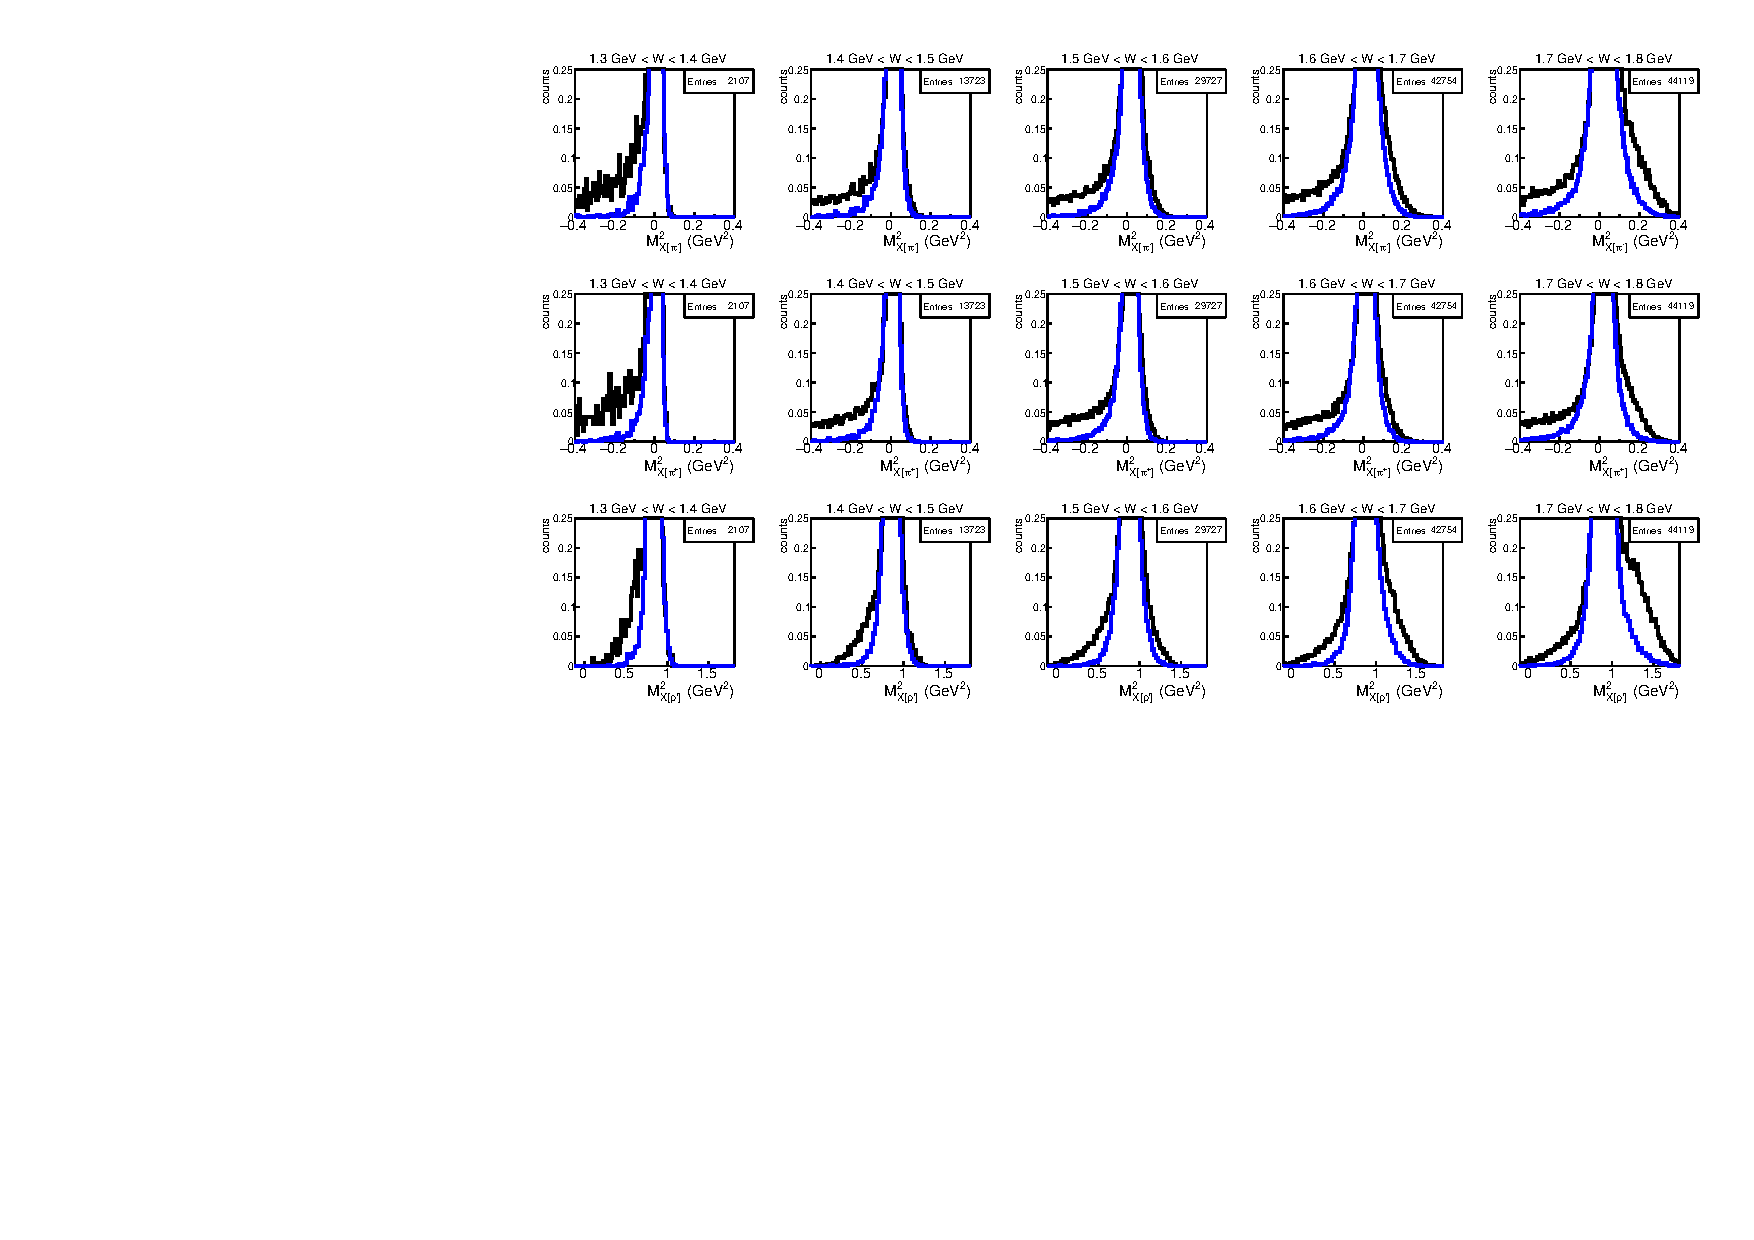
\includegraphics[width=\textwidth]{pictures/fsi_discuss/all_mass_stat.pdf}}
\end{center}
\caption{\small Distributions of the quantities $M^{2}_{X[\pi^{-}]}$ (first row), $M^{2}_{X[\pi^{+}]}$ (second~row), and $M^{2}_{X[p']}$ (third row) defined in (or analogously to) Eq.~\eqref{eq:excl_top_quant2}. The relative spread of events~with FSI in five 100-MeV-wide bins in $W$ is demonstrated by the mismatch between the experimental (black) and the simulated (blue) histograms. The distributions are plotted~for~events from the fully exclusive topology and normalized in a way that the peak maxima are equal~to one. They are however zoomed in on the range [0,~0.25] on the $y$-axis to~better visualize the mismatch. The shown statistics corresponds to the unzoomed experimental distributions.}
\label{fig:all_mass}
\end{figure}

The distributions from Fig.~\ref{fig:all_mass} illustrate the cumulative contribution from FSI for the $\pi^{+}$ and proton (first row), $\pi^{-}$ and proton (second row), and $\pi^{+}$ and $\pi^{-}$ (third row). They share several global distinctive features. Specifically, for all distributions the left-side tail does not show any $W$ dependence staying on a constant substantial level throughout the whole $W$ range, being though a bit more prominent in the first bin. The tail at the right side, in turn, is absent for low $W$ and gradually increases as $W$ grows. This is thought to be driven by the following reasons. 


First, the left-side tail was proven to contain a large portion of events, in which non-relativistic protons lose their momentum through FSI. Meanwhile, the majority of registered protons in this experiment is non-relativistic, which ensures the stable saturation of the left-side tail throughout the whole $W$ range (for distributions from the first and second rows). At the same time, the right-side tail was proven to contain a large portion of events, in which relativistic hadrons (which are mostly pions) lose their momentum through FSI. This portion, in turn, grows with $W$, which leads to gradual emergence of the right-side tail. %Note also that the Fermi smearing promote


The slight prominence of the left-side tail and the complete absence of the tail at the right in the first $W$ bin is then due to (i) the abundance of the low-momentum hadrons near the threshold, (ii) the deficiency of the high-momentum hadrons there, and (iii) the most prominent asymmetry of the Fermi smearing in this region.


Once the main similarities of the distributions from Fig.~\ref{fig:all_mass} are addressed, one can discuss their differences and other related features. Thus, the right-side tail, although keeping nearly the same structure for all distribution types, demonstrates different intensity manifestation, which is the smallest for $M^{2}_{X[\pi^{+}]}$ (second row), greater for $M^{2}_{X[\pi^{-}]}$ (first row), and the largest for $M^{2}_{X[p']}$ (third row). This allows for the following conclusion: in the considered event sample the cumulative amount of relativistic $\pi^{-}$ and protons that lose their momentum in FSI is smaller than that of $\pi^{+}$ and protons, which in turn is smaller than the corresponding amount of $\pi^{+}$ and $\pi^{-}$. Note that this conclusion is very likely to be dependent on the experimental conditions.

%\everypar{\looseness=-1}
The next feature is related to the left-side tail, which although keeping generally the same $W$ dependence and intensity manifestation for all distributions, demonstrates some structural variations. Thus, for the first two rows, the left-side tail is long and its structure is flat, while for the third row the tail is shorter (relative to the main peak) and has a steeper shape. This observation allows for the following interesting conclusion. 


The point is that distributions from the first and second rows include the contributions from the proton FSI as well as from FSI of one type of pion, whereas the distributions from the third row isolate the FSI contribution from both pion types. Therefore, for the first two rows, the left-side tail is dominated with events, in which non-relativistic protons lose the momentum. Meanwhile, for the third row, where such events are not present, the left side-tail is populated with events, in which (i)  relativistic pions gain their momentum and (ii) non-relativistic pions lose their momentum. Both these event types do not happen very often, so the $M^{2}_{X[p']}$ distributions offer a great opportunity to isolate them. One should also keep in mind that some part of the events in the left tail is tossed there from the right side by the Fermi smearing.

Note that the distributions from the first and second rows contain the aforementioned two types of rarer FSI events as well, but only for one type of pion, which means around a half of them. Their manifestation then turns out to be masked by events with the momentum loss of non-relativistic protons, which is the dominant type of FSI events in the left-side tail.


Additionally, from the structure of the left-side tails of distributions in Fig.~\ref{fig:all_mass}, one can suggest that events with proton FSI are subject to a larger spread along the $x$-axis than events with pion FSI. This observation is confirmed by Ref.~\cite{note_mm_distr} as it demonstrates that, when the same variation in the momentum magnitude for pions and protons is considered, the distortions in the $M^{2}_{X[\pi^{-}]}$ distributions caused by the proton FSI are larger (i.e. their structure is flatter and the spread along the $x$-axis is of a larger extent) than those for the case of the pion FSI.


\newpage

\section{FSI in topologies with a missing hadron}


As follows from the findings revealed above, the set of missing quantities $M^{2}_{X[i]}$ (where $i$ corresponds to the missing hadron) offers great opportunities for studying kinematic manifestations of FSI effects because each $M^{2}_{X[i]}$ is capable of isolating the FSI contributions from the corresponding pair of registered hadrons. However, this advantage is mostly related to the fully exclusive topology, where all three available quantities $M^{2}_{X[i]}$ are auxiliary with respect to the primary quantity $M^{2}_{X[0]}$ that incorporates information of all registered final hadrons and hence is typically used to isolate the reaction channel. Meanwhile, for topologies with one unregistered hadron, the corresponding quantity $M^{2}_{X[i]}$, being the only one available, has to be used for the channel identification. Under these conditions, the aforementioned ability of $M^{2}_{X[i]}$ to isolate FSI contributions from the pair of registered hadrons results in some complications, as described below.


In general, when dealing with topologies with one unregistered hadron, the four-momentum of this hadron is typically reconstructed as missing using the four-momenta of registered particles and then the exclusivity cut on the corresponding distribution of $M^{2}_{X[i]}$ is performed for isolating the channel. The success of this conventional method is based on the fact that particles produced in one reaction are not independent as they share the same reaction kinematics, which imposes some reaction-specific constraints on their four-momenta. As a result, the particle four-momenta entangle, making the information on one particle to be incorporated into the kinematics of the others. 


This method, however, works smoothly only for quasi-free events, while for events with FSI it, in fact, gives an incorrect output because (as was already mentioned) once participating in FSI, hadrons do not further keep the kinematics of the initial reaction and formally can no longer be attributed to this reaction. %Here several interesting aspects come into play, which are addressed below.


To be more specific, the following three possibilities can be distinguished for events from the topologies with an unregistered hadron (assuming that  only one final hadron in an event interacts with the neutron).


\begin{itemize}
\item[1.] All final hadrons in an event avoided FSI with the neutron. Then this event is a true quasi-free event and the four-momentum of the unregistered hadron can be successfully reconstructed as missing by means of the conventional procedure.
\item[2.] The unregistered hadron avoided FSI, while one of the registered hadrons interacted in the final state, changing in this way its four-momentum and hence losing its kinematic affiliation to the initial reaction. This does not allow the proper reconstruction of the missing hadron four-momentum, causing the event to contribute to the FSI-background in the distributions of $M^{2}_{X[i]}$.
\item[3.] The unregistered hadron experienced FSI with the neutron and the registered hadrons avoided them. In this case, the missing four-momentum of the unregistered hadron corresponds to its four-momentum before FSI. Such an event is then falsely treated as quasi-free.
\end{itemize}


The given disposition reveals some important issues. First, the hadron four-momentum turns out to be the only one source of information on FSI (with the spectator nucleon) this hadron may undergo. If the hadron is not registered, the information on its interaction turns out to be lost beyond reconstruction as the other particles are not aware of this happening.

The next important thing to mention is that in reactions off bound nucleons, topologies with a missing hadron are revealed to suffer from miscounting of both quasi-free events and events with FSI as their separation is inaccurate. Specifically, the amount of quasi-free events is systematically overestimated because events of the third type are considered to be quasi-free, whereas they are actually events with FSI. Although the overestimation is not expected to be dramatic, this issue should be carefully considered as it may have an impact on the interpretation of the final results of a data analysis.

With that said, one can pay closer attention to the $\pi^{-}$-missing topology of this particular analysis\footnote[9]{Note that the $\pi^{-}$-missing topology is the main analysis topology, the fully exclusive topology is a complementary one, while the two other topologies are not used. See more details in Sect.~\ref{Sect:excl_cut}.}. Figure~\ref{fig:main_top} shows the distributions of the missing quantity $M^{2}_{X[\pi^{-}]}$ plotted for this topology. The relative spread of events with FSI in five 100-MeV-wide bins in $W$ is demonstrated by the mismatch between the experimental (black) and the simulated (blue) histograms. The distributions are normalized in a way that the peak maxima are equal to one and then zoomed in on the range [0,~0.25] on the $y$-axis, to better visualize the mismatch and for consistency with the distributions~in~Fig.~\ref{fig:all_mass}.
\begin{figure}[!ht]
\begin{center}
\framebox{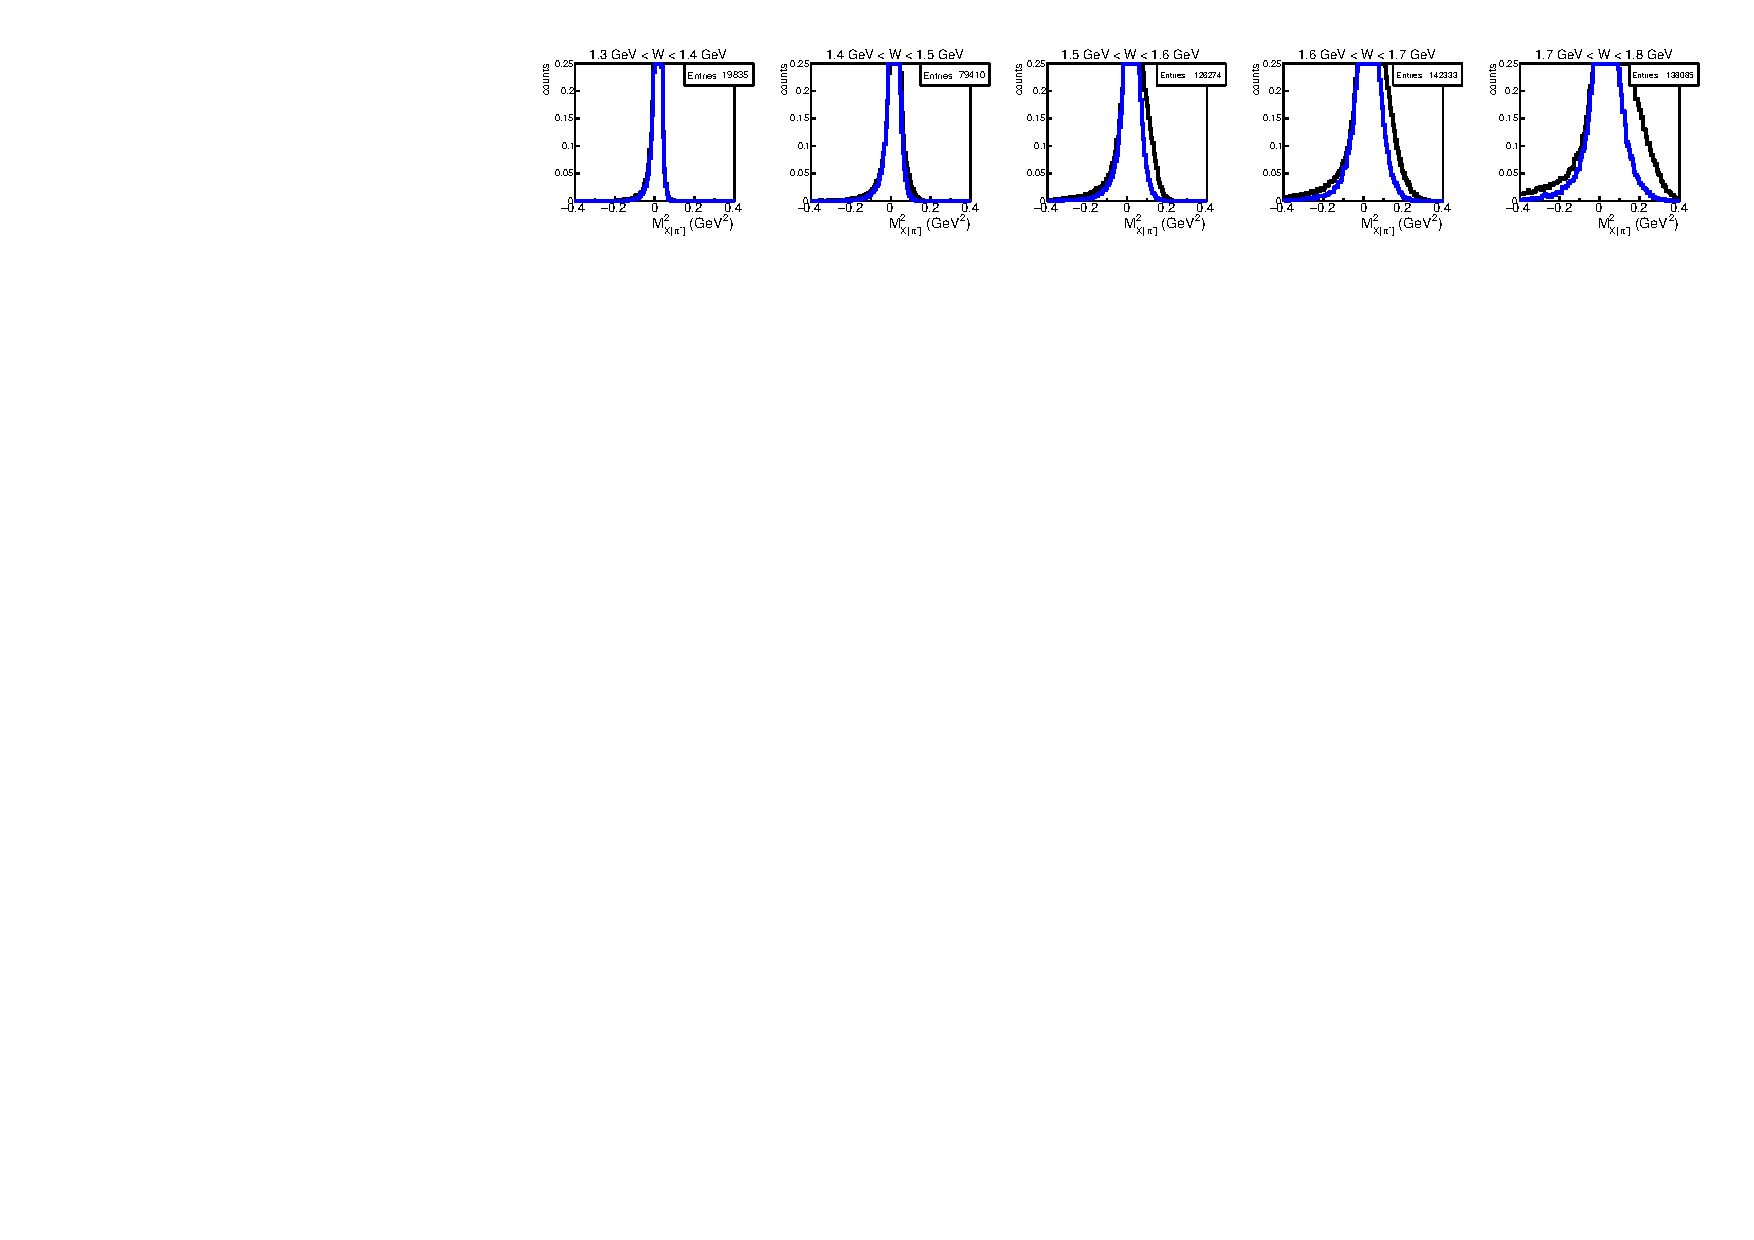
\includegraphics[width=\textwidth]{pictures/fsi_discuss/main_top_mmsq_stat.pdf}}
\end{center}
\caption{\small Distributions of the missing quantity $M^{2}_{X[\pi^{-}]}$ plotted for the $\pi^{-}$-missing topology. The relative spread of events with FSI in five 100-MeV-wide bins in $W$ is demonstrated by the mismatch between the experimental (black) and the simulated (blue) histograms. The distributions are normalized in a way that the peak maxima are equal to one and then zoomed in on the range [0,~0.25] on the $y$-axis, to better visualize the mismatch. The presented statistics corresponds to the unzoomed experimental distributions.}
\label{fig:main_top}
\end{figure}

The distributions in Fig.~\ref{fig:main_top} reflect the contributions from FSI of the proton and $\pi^{+}$ and do not include the information on the $\pi^{-}$ interactions, being analogous in that sense to the distributions in the first row of Fig.~\ref{fig:all_mass} related to the fully exclusive topology. This analogy advantages their comparison.



As seen in Fig.~\ref{fig:main_top}, for $W\lesssim$~1.5~GeV no significant mismatch between the experimental (black) and the simulated (blue) distributions is present. The explanation of this effect, which is not observed in the first row of Fig.~\ref{fig:all_mass}, lies in the kinematic differences between the two topologies.


The point is that the $\pi^{-}$-missing topology contains mostly events with negative pions of low momentum as they escape through the forward acceptance hole. Meanwhile, the fully exclusive topology includes events, in which the $\pi^{-}$ momentum varies from moderate to high as they manage to be registered. Consequently, in the fully exclusive topology, the momenta of the proton and the $\pi^{+}$ are on average lower than in the $\pi^{-}$-missing topology. This situation turns out to influence the relative spread of FSI affected events.  

First, the dominant contribution to the left-side tail of the $M^{2}_{X[\pi^{-}]}$ distribution was shown to be formed by FSI events, in which non-relativistic protons lose their momentum. Meanwhile, the $\pi^{-}$ topology happens to lack this kind of events as their major part belongs to the fully exclusive topology.

Another consequence is related to the fact that the probability to interact in the final state depends on the relative velocity of the interacting hadrons, i.e. for slower traveling hadrons the chance to interact is higher than for rapid hadrons. As a result, the two topologies turn out to have different distributions of the interaction probability among the final hadrons due to the difference in their momenta. Specifically, negative pions attributed to the $\pi^{-}$-missing topology have higher probability to interact than those attributed to the fully exclusive topology. Meanwhile, for protons and positive pions the situation is the opposite, i.e. their chances to interact are higher for the fully exclusive topology.

Therefore, if compared with the $\pi^{-}$-missing topology, the fully exclusive one contains larger number of events with alterations in the proton and $\pi^{+}$ four-momenta caused by FSI, which results in more disturbances seen in the $M^{2}_{X[\pi^{-}]}$ distributions as these four-momenta are used to calculate this missing quantity. 

At the same time, the $\pi^{-}$-missing topology accumulates more events with the $\pi^{-}$ FSI than the fully exclusive topology. However, the quantity $M^{2}_{X[\pi^{-}]}$ does not reflect the information on the $\pi^{-}$ interactions as its four-momentum is excluded from the calculation of this quantity. This, in turn, promotes the presence of falsely defined quasi-free events in the $M^{2}_{X[\pi^{-}]}$ distributions, and their amount correlates with the aforementioned probability of the $\pi^{-}$ interactions. This effect causes the distributions of the $\pi^{-}$-missing topology to acquire fewer distortions than their fully exclusive analogues, with the maximum difference achieved near the threshold.



The combination of these effects explains the good match between the experimental and simulated distributions of $M^{2}_{X[\pi^{-}]}$ observed in the $\pi^{-}$-missing topology for $W\lesssim$~1.5~GeV, which is not achieved in the fully exclusive topology. %Besides this, it also explains the shape and $W$ behavior of both left and right tails in the distributions in Fig.~\ref{fig:main_top}.

A further comparison of distributions in Figs.~\ref{fig:all_mass} and~\ref{fig:main_top} also reveals that the left-side tail of the $M^{2}_{X[\pi^{-}]}$ distributions in the $\pi^{-}$-missing topology differs from its analogue from the fully exclusive topology both in intensity and in $W$ dependence. Specifically, being completely absent near the threshold, it shows a constant, but rather mild growth with $W$, staying on a still very moderate level even in the last $W$ bin. Meanwhile, the right-side tails for both cases are very alike, though for the $\pi^{-}$-missing topology it shows more intensive growth with $W$. 


\everypar{\looseness=-1}
The understanding again lies in the fact that the $\pi^{-}$-missing topology lacks low momentum protons and $\pi^{+}$, having instead an excess of high-momentum hadrons of these types, with all the consequences addressed above. This causes the lack of FSI events with the momentum loss for non-relativistic hadrons and the corresponding abundance of events with the momentum loss for relativistic hadrons, which in turn results in the suppression of the left-side tail and some affluence of the tail at the right.


It is also important to pay closer attention to the issue with the falsely defined quasi-free events that contribute to the $M^{2}_{X[\pi^{-}]}$ distributions of the $\pi^{-}$-missing topology. As was already stated above, in this topology many unregistered $\pi^{-}$ experience FSI due to their very low momentum, leaving the registered protons and $\pi^{+}$ of the corresponding event to remain quasi-free. This effect is very pronounced near the threshold and is mitigated with growing $W$ as proven by the gradually emerging disturbances in the $M^{2}_{X[\pi^{-}]}$ distributions in Fig.~\ref{fig:main_top}, which indicate more registered hadrons experiencing FSI and hence more quasi-free unregistered $\pi^{-}$. As a result, the amount of falsely defined quasi-free events is maximal near the reaction threshold and declines for higher $W$. Although such a miscounting itself is inevitable for any topology with a missing hadron in reactions off bound nucleons, the amount of the miscounted events, and its spread along $W$ is to a high degree determined by experimental conditions.  


\section{Resonance formation in pion-neutron FSI}
\label{Sect:resonance_fsi}

So far the main attention of this investigation has concentrated on the momentum alterations that final hadrons undergo via FSI as a universal criterion for distinguishing events with FSI from regular quasi-free events, without any particular focus on the interaction mechanism itself. Meanwhile, the strong interaction, which drives FSI, offers a very broad spectrum of these mechanisms. Although this study mostly concentrates on kinematic effects and hence does not claim any attempt of a full description of any particular mechanism, it is interesting to dig into one more promising direction in order to fully exploit the opportunities provided by this experimental dataset for a better understanding of FSI.

First, it is worthwhile to recall that in the analyzed reaction, FSI are dominated by elastic scattering of final hadrons off spectator neutrons, i.e. by interactions, in which (i) the quantum numbers of the participating hadrons do not change and (ii) no new particles are produced. Inelastic mechanisms, which do not satisfy these two criteria, are meanwhile less pronounced. 


%The process, in which a final hadron ($h$) couples with the spectator neutron ($n$), producing nucleon resonances ($R$) in the intermediate state, can be represented as $hn \rightarrow R \rightarrow \sum_{i} h'_{i}$, where $h'_{i}$ are the resonance decay products, which are registered by the detector afterwards.


\everypar{\looseness=-1}
This particular Section examines the process, in which a final hadron ($h$) couples with the spectator neutron ($n$), producing nucleon resonances ($R$) in the intermediate state. This can be represented as $hn \rightarrow R \rightarrow \sum_{i} h'_{i}$, where $h'_{i}$ are the resonance decay products, which are registered by the detector afterwards. In this situation very interesting things may happen, i.e. depending on the resonance decay mode, the registered hadrons may differ from those that form the resonance, both in their type and/or amount. Such processes then can contribute to both elastic and inelastic FSI parts.

\everypar{\looseness=-1}
To dig into this issue, advantages offered by the fully exclusive topology can again be of use. Specifically, with the four-momenta of all final hadrons available, one can reconstruct the four-momentum of the spectator neutron as missing. Although such reconstruction is inaccurate for events with FSI and also suffers from the Fermi smearing, the resulting four-momentum still suits the purpose of this examination. Specifically, the following set of the invariant masses can be calculated,%\vspace{-0.75em}
\begin{equation}\tag{9.2}
\begin{aligned}
&M_{n'\pi^{-}}&=~& \sqrt{(P_{n'}^{\mu} + P_{\pi^{-}}^{\mu})^{2}}, & \\ \label{eq:fsi_invmasses}
&M_{n'\pi^{+}}&=~& \sqrt{(P_{n'}^{\mu} + P_{\pi^{+}}^{\mu})^{2}}, & \text{~~~and} \\ 
&M_{n'p'}&=~& \sqrt{(P_{n'}^{\mu} + P_{p'}^{\mu})^{2}}, &\\
\end{aligned}  
\end{equation}  
where $P_{n'}^{\mu}$ is the four-momentum of the spectator neutron calculated as missing under the target-at-rest assumption, while $P_{\pi^{-}}^{\mu}$, $P_{\pi^{+}}^{\mu}$, and $ P_{p'}^{\mu}$ are the four-momenta of the final hadrons registered by the detector.

Figure~\ref{fig:inv_m} shows the distributions of the invariant masses $M_{n'\pi^{-}}$ (first row), $M_{n'\pi^{+}}$ (second row), and $M_{n'p'}$ (third row) from Eqs.~\eqref{eq:fsi_invmasses} plotted for the experimental data (black histograms) and the regular Monte-Carlo simulation (blue histograms). The dashed green histograms are auxiliary as they correspond to the same simulation, but with the cross section weights ignored, which means that phase-space distributions are assumed for all kinematic variables instead of the regular realistic distributions~\cite{twopeg,twopeg-d}. These green histograms are intended to visualize the impact of the assumptions for the cross section shape implemented into the event generator~\cite{twopeg-d}.

\newpage
In general, invariant mass distributions are very helpful in checking for the presence of an unstable particle, whose decay causes the emission of particles involved in the invariant mass calculation. If this is the case, then the invariant mass distributions acquire a peak at the position of the mass of this unstable particle. 

Therefore, if an unstable particle was formed during FSI, then it should be seen as an agglomeration of events with FSI in the corresponding invariant mass distribution, which again can be visually spotted as a mismatch between the experiment and the simulation. Keeping that in mind, one can now examine the invariant mass distributions shown in Fig.~\ref{fig:inv_m}. Note that in Fig.~\ref{fig:inv_m} all histograms are normalized in a way that their peak maxima are equal to one. 

\begin{figure}[!ht]
\begin{center}
\framebox{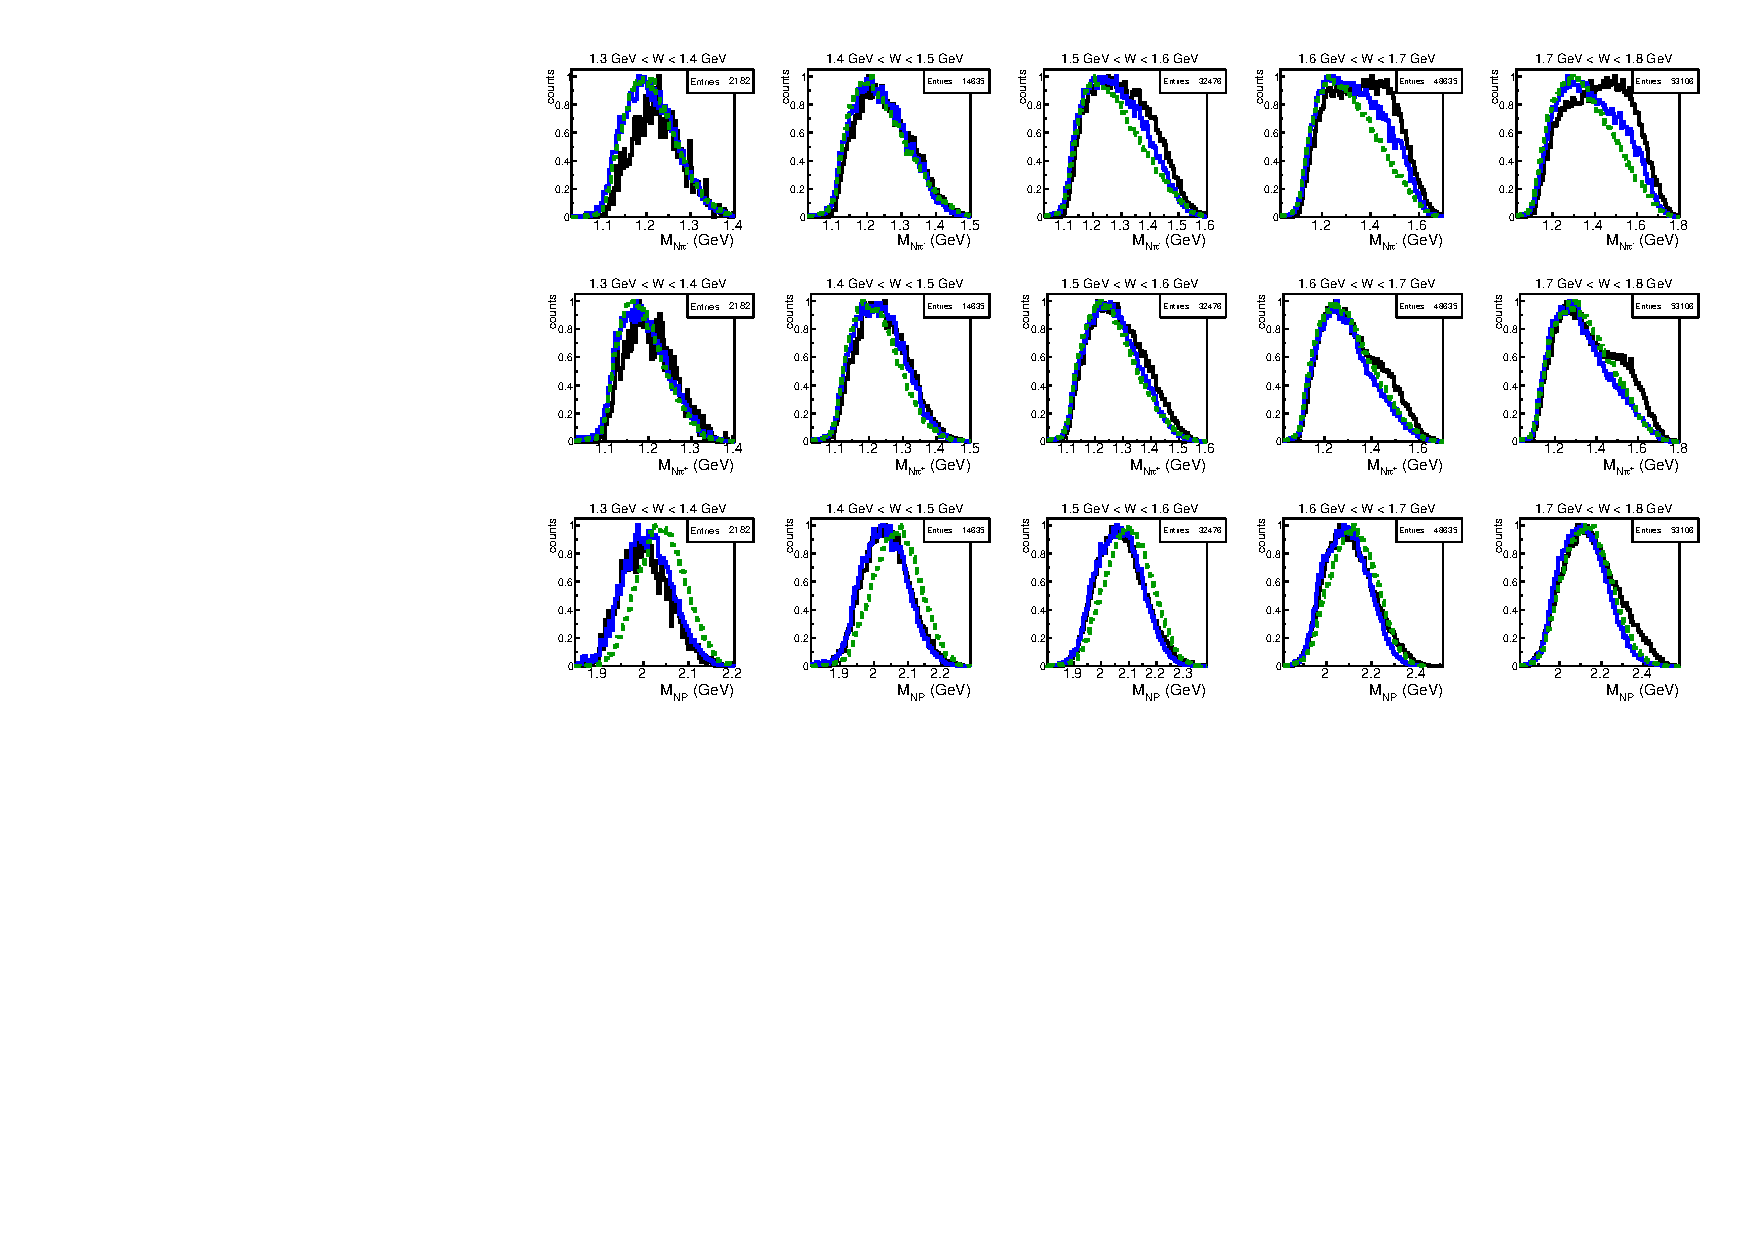
\includegraphics[width=\textwidth]{pictures/fsi_discuss/inv_m_stat.pdf}}
\end{center}
\caption{\small Distributions of the invariant masses $M_{n'\pi^{-}}$ (first row), $M_{n'\pi^{+}}$ (second row), and $M_{n'p'}$ (third row) from Eqs.~\eqref{eq:fsi_invmasses} plotted for experimental data (black histograms) and regular Monte-Carlo simulation (blue histograms). The dashed green histograms are auxiliary as they correspond to the same simulation, but with the cross section weights ignored, which means that phase-space distributions of all kinematic variables are used instead of the regular realistic distributions~\cite{twopeg,twopeg-d}. The mismatch between the data and the simulation is indicative of the agglomeration of events with FSI. All histograms are normalized in a way that the peak maxima are equal to one. The presented statistics corresponds to the experimental data.}
\label{fig:inv_m}
\end{figure}

The final proton and the spectator neutron are not expected to couple to each other with the formation of an unstable particle in the intermediate state as both of them are baryons. This conclusion is confirmed by the invariant mass distributions shown in the third row of Fig.~\ref{fig:inv_m}, where the experimental and the simulated histograms agree with each other, both replicating the shape typical for the case of the phase-space distribution~of~all~kinematic~variables.


The situation is however different for the invariant masses $M_{n'\pi^{-}}$ and $M_{n'\pi^{+}}$ as the neutron can willingly couple to either $\pi^{-}$ or $\pi^{+}$ forming a nucleon resonance, and the resonance mass is then determined by the cumulative energy of the coupled pair. Thus, for low $W$, the formation of the $\Delta$ resonances is only possible, while for higher $W$ other resonances with larger masses will compete for the formation. 

The visual spotting of the $\Delta$ resonances in the distributions of the invariant masses comes meanwhile with some difficulties. They originate from the fact that $\Delta$ resonances peak around $\sim$1.2~GeV, and the phase-space invariant mass distribution behaves similarly at low $W$. Therefore, as long as the width of the invariant mass distribution is comparable with the width of the $\Delta$ resonance (which is around 120~MeV), it is difficult to visually distinguish between resonant and non-resonant events as they form the same invariant mass structure. This effect is seen in the first and second rows of Fig.~\ref{fig:inv_m}, where the experiment matches the simulation for $W\lesssim$~1.6~GeV, although the formation of $\Delta$ resonances is highly expected.

For higher $W$ however the situation simplifies as the spread of the invariant mass distribution is now sufficient for observing the structures with lower width. Thus, for $W\gtrsim$1.6~GeV the observed mismatch between the data and the simulation reveals the agglomeration of events with FSI at invariant mass values $\gtrsim$1.4~GeV, which correspond to the masses of the resonances from the second resonance region. The contribution from the $\Delta$ resonance is, however, still hard to judge due to the overall normalization of the distributions.

Thus, the invariant mass distributions in Fig.~\ref{fig:inv_m} may serve as evidence that both $\pi^{-}$ and $\pi^{+}$ do couple to the spectator neutron in the final state with the formation of several resonances, including those from the second resonance region. And moreover, the chance for the neutron and $\pi^{-}$ pair to originate from the decay of the resonances from the second resonance region is much higher than that for the neutron and $\pi^{+}$ pair as confirmed by the much larger mismatch observed in the $M_{n'\pi^{-}}$ distributions (first row) comparing with the $M_{n'\pi^{+}}$ distributions (second row).



These findings allow for several interesting processes to be traced. First, for the neutron to pion coupling with the formation of $\Delta$ resonances, the following options are available. If the neutron couples to the $\pi^{-}$, then the $\Delta^{-}$(1232) resonance is formed, which then decays with the emission of the same hadron pair that was involved in its formation (the original momenta are however not kept). Meanwhile, if the neutron couples to the $\pi^{+}$, then the $\Delta^{+}$ resonance is formed, which has two decay options, i.e. either to the $n\pi^{+}$ or $p\pi^{0}$ final states. In the former case, the emitted hadrons are of the same type as the initial, with the different momentum though. However, in the latter case, both emitted hadrons differ from those in the FSI initial state.

The situation complicates further if the formation of the resonances of the second resonance region is considered. In this case, the decaying resonance may emit mesons different than pions (such as $\rho$, $\sigma$, etc.) or even baryons different than nucleons (such as $\Lambda$, $\Sigma$). The latter is however not expected to happen in this experiment due to its low beam energy, which does not allow for the formation of the resonances with this decay mode as they have too large masses.

Additionally, the resonances of the second resonance region can produce more than two decay products, and the decay to the $N\pi\pi$ final state is the most probable mode of this kind. In this case the resonance decay products differ from the hadrons involved in its formation not only in their type but also in amount.%, which further entangles the situation. 

Besides this, one more impact of FSI on the reaction final state becomes evident, when considering the resonances of the second resonance region decaying to the $N\pi\pi$ final state. In this case, several options for the types of the nucleon and the pions in the FSI final state are in general possible with the following two processes being the most remarkable, i.e. $n\pi^{-}\rightarrow R\rightarrow n\pi^{-}\pi^{0}$ and $n\pi^{+}\rightarrow R\rightarrow n\pi^{+}\pi^{0}$, where $R$ corresponds to a resonance. Although in these processes the neutron and pion maintain their types throughout the resonance formation and decay, their momenta are now affected beyond the level of individual alterations, i.e. their total momentum is not conserved as it leaks out via the $\pi^{0}$ emission.


Thus, one can conclude that the neutron-pion coupling with the resonance formation, which takes place during FSI, in general resolves in the following options\footnote[10]{Note that all these options are also relevant for interactions of the final hadrons with each other.},\vspace{-0.25em}
\begin{itemize}
\item the types of the particles involved in FSI are kept, their momenta alter but the total momentum of the interacting pair is conserved,
\item the types of the particles involved in FSI are kept, their momenta alter, but the cumulative momentum leaks via the emission of an additional particle, and 
\item the types of the particles involved in FSI are not kept.
\end{itemize}

The first option then corresponds to elastic interactions, while the second and the third belong to inelastic. It is also essential that manifestations of these options in analyses of experimental data off bound nucleons have some specificities, which are briefly addressed below.


Specifically, events that correspond to the first option turn out to be kinematically identical to those events, in which pions change their momenta through non-resonant rescattering off the spectator nucleon as in both cases pions experience either momentum gain or loss. Therefore, events of both kinds share the same kinematic behavior, which was discussed above.


If the process with the momentum leak occurs (the second option), then the chances are high that the corresponding $\pi^{-}$ or $\pi^{+}$, if registered, would still be attributed to the original channel during the data analysis, especially taking into account the very poor efficiency of the $\pi^{0}$ registration in CLAS. In that case, such an event can not be distinguished from FSI events with the momentum alterations that conserve the total momentum of the interacting pair, like in the process $n\pi^{-}\rightarrow \Delta^{-}\rightarrow n\pi^{-}$ or in a simple momentum exchange, which are events of the first type. This is because the neutron (which is withal not registered) is extrinsic with respect to the original exclusive channel (which happens off protons) and hence is not included in its kinematics. Therefore, from the point of view of the original reaction, events with the momentum leak are FSI events with the pion momentum loss and hence comply with the patterns derived above for such kind of events.


\everypar{\looseness=-1}
Meanwhile, the third scenario leads to the modification of the final state of the original reaction due to FSI, which causes the registered particles to be attributed to a wrong exclusive channel with the consequence of miscounting events selected for a particular reaction. This problem can be however resolved to a very high degree on the level of the exclusivity cut on a missing mass distribution that is typically used for the channel identification. The majority of falsely defined events will not survive this cut because such events will fail to contribute to the main missing mass peak, as they do not keep the kinematics inherent for the channel that is subject to the selection.


\everypar{\looseness=-1}
At this point, the examination being conducted seems to exploit to a very high degree the opportunities offered by this experimental dataset for a better understanding of FSI effects, which occur in the reaction of the double-pion production off protons in deuterium. Therefore, considering the objectives set to this chapter being fulfilled, one can conclude the whole discussion of FSI effects, which accompanies the main analysis. 




%----------------------------------------------------

%Note: momentum and angles are in lab system. 
%And momentum and angles for quasi-free events are actual, while for events with FSI are changed by FSI. 
%And where FSI are significant $-->$ left missing mass tail $-->$ momentum gain.
%It is a qualitative but not a quantitative estimation.


%FSI$->$W-dependence+angular dependence=topology dependence
%Consider two topologies separately
%Fully exclusive suits best. Let's start from it
%Missing momentum distributions allow to judge. Slices in theta angles. ...

%Set of invariant masses from the fully exclusive topology. Are particles' productions possible?

%Then pim miss. Interaction with missing hadron! $->$ free proton?

%Free proton + less than 5\% interaction $->$ Ref to CLAS-note $->$ GPP parameters. $->$ 


%Free proton cross sections are convoluted with less than 5\% FSI, and so do these cross sections $->$ benefit from same GPP parameters.

%One reason of mismatch between actual and simulated CLAS resolution and the consequent need of GPP $->$ FSI. 


%-----------------------------!!!!!!!!!!!!!!!!!!!!!---------------------------
%Theta vs p $-->$ protons.
%explanation of Gaussian shape of FSI background in the exclusivity cut.%?????


